% !TeX program = pdflatex
% !BIB program = biber
% Dokument A: ausführliche Dokumentation von Modul 4 (Behavior Cloning).
% Bauen:  latexmk   (im Ordner Ausfuehrlich, Ausgabe nach build/)
\documentclass[
  a4paper,
  12pt,
  oneside,
  parskip=half,
  bibliography=totoc,
  listof=totoc,
  numbers=noenddot
]{scrreprt}

% Gemeinsame Präambel der M4-Dokumente (übernommen aus thesis/main.tex, damit die Integration einfach bleibt).
% Wird aus einem Unterordner eingebunden; Pfade sind relativ zu diesem Unterordner.
% --- Sprache und Schrift -------------------------------------------------------
\usepackage[T1]{fontenc}
\usepackage[utf8]{inputenc}
\usepackage[ngerman]{babel}
\usepackage{lmodern}
\usepackage{microtype}
\usepackage[autostyle=true,german=quotes]{csquotes}

% --- Layout --------------------------------------------------------------------
\usepackage[left=3cm,right=2.5cm,top=2.5cm,bottom=2.5cm]{geometry}
\usepackage{setspace}
\onehalfspacing

% --- Inhalte -------------------------------------------------------------------
\usepackage{graphicx}
\graphicspath{{abbildungen/}{../../../../../thesis/figures/}}
\usepackage{amsmath,amssymb}
\usepackage{siunitx}
\sisetup{locale=DE}
\usepackage{booktabs}
\usepackage{tabularx}
\usepackage{listings}
\lstset{basicstyle=\ttfamily\small,breaklines=true,frame=single,language=Python,
        numbers=left,numberstyle=\tiny,showstringspaces=false}
\usepackage{xcolor}
\usepackage{acro}
\usepackage{tikz}
\usetikzlibrary{arrows.meta,positioning,automata,fit,shapes.geometric,calc}
% Ablaufdiagramme (Programmablaufplan)
\tikzset{
  pap/.style={node distance=6mm and 10mm, font=\small},
  pap term/.style={draw, rounded corners=3mm, fill=black!8, align=center, minimum height=7mm,
                   inner xsep=3mm},
  pap proc/.style={draw, fill=white, align=center, text width=#1, minimum height=8mm},
  pap proc/.default=64mm,
  pap dec/.style={draw, diamond, aspect=2.6, fill=black!3, align=center, inner sep=1pt},
  pap arr/.style={-{Stealth[length=2.2mm]}, thick},
  pap lbl/.style={font=\scriptsize, fill=white, inner sep=1pt},
  pap good/.style={pap term, fill=green!12},
  pap bad/.style={pap term, fill=red!10},
}
\usepackage{algorithm}
\usepackage{algpseudocode}
\floatname{algorithm}{Algorithmus}
\algrenewcommand\algorithmicrequire{\textbf{Eingabe:}}
\algrenewcommand\algorithmicensure{\textbf{Ausgabe:}}
\algrenewcommand\algorithmicif{\textbf{wenn}}
\algrenewcommand\algorithmicthen{\textbf{dann}}
\algrenewcommand\algorithmicelse{\textbf{sonst}}
\algrenewcommand\algorithmicfor{\textbf{für}}
\algrenewcommand\algorithmicforall{\textbf{für alle}}
\algrenewcommand\algorithmicdo{\textbf{tue}}
\algrenewcommand\algorithmicwhile{\textbf{solange}}
\algrenewcommand\algorithmicreturn{\textbf{gib zurück}}
\algrenewcommand\algorithmicfunction{\textbf{Funktion}}
\algrenewcommand\algorithmicprocedure{\textbf{Prozedur}}
\algrenewcommand\algorithmicend{\textbf{Ende}}
\algrenewcommand{\algorithmiccomment}[1]{\hfill$\triangleright$ #1}
\renewcommand{\listalgorithmname}{Algorithmenverzeichnis}
\usepackage[colorinlistoftodos,textsize=footnotesize]{todonotes}

% --- Literatur (IEEE) ----------------------------------------------------------
\usepackage[backend=biber,style=ieee,dashed=false]{biblatex}
\addbibresource{../../../../../thesis/references.bib}
\addbibresource{../m4.bib}

% --- Links (zuletzt laden) -----------------------------------------------------
\usepackage[hidelinks]{hyperref}
\usepackage[ngerman]{cleveref}
\crefname{algorithm}{Algorithmus}{Algorithmen}


% --- Abkürzungen: die der Gesamtarbeit plus M4-spezifische ---------------------
\DeclareAcronym{ocr}{short=OCR, long=Optical Character Recognition}
\DeclareAcronym{tcp}{short=TCP, long=Tool Center Point}
\DeclareAcronym{ks}{short=KS, long=Koordinatensystem}
\DeclareAcronym{ptp}{short=PTP, long=Point-to-Point}
\DeclareAcronym{lin}{short=LIN, long=Linearbewegung}
\DeclareAcronym{roi}{short=ROI, long=Region of Interest}
\DeclareAcronym{cnn}{short=CNN, long=Convolutional Neural Network}
\DeclareAcronym{cobot}{short=Cobot, long=kollaborativer Roboter}
\DeclareAcronym{api}{short=API, long=Application Programming Interface}
\DeclareAcronym{gui}{short=GUI, long=Graphical User Interface}
\DeclareAcronym{hsv}{short=HSV, long=Hue{,} Saturation{,} Value}
\DeclareAcronym{csv}{short=CSV, long=Comma-Separated Values}
\DeclareAcronym{lan}{short=LAN, long=Local Area Network}
\DeclareAcronym{bc}{short=BC, long=Behavior Cloning}
\DeclareAcronym{vm}{short=VM, long=virtuelle Maschine}
\DeclareAcronym{ik}{short=IK, long=inverse Kinematik}
\DeclareAcronym{gpu}{short=GPU, long=Graphics Processing Unit}
\DeclareAcronym{rms}{short=RMS, long=Root Mean Square (quadratischer Mittelwert)}
\DeclareAcronym{usb}{short=USB, long=Universal Serial Bus}

% Zusätzliche Abkürzungen nur für die M4-Dokumente (nicht doppelt zu 00_abkuerzungen.tex).
\DeclareAcronym{dp}{short=DP, long=Diffusion Policy}
\DeclareAcronym{ddpm}{short=DDPM, long=Denoising Diffusion Probabilistic Model}
\DeclareAcronym{ddim}{short=DDIM, long=Denoising Diffusion Implicit Model}
\DeclareAcronym{dart}{short=DART, long=Disturbances for Augmenting Robot Trajectories}
\DeclareAcronym{dagger}{short=DAgger, long=Dataset Aggregation}
\DeclareAcronym{ou}{short=OU, long=Ornstein-Uhlenbeck}
\DeclareAcronym{ema}{short=EMA, long=Exponential Moving Average}
\DeclareAcronym{fk}{short=FK, long=Vorwärtskinematik}
\DeclareAcronym{urdf}{short=URDF, long=Unified Robot Description Format}
\DeclareAcronym{rpc}{short=RPC, long=Remote Procedure Call}
\DeclareAcronym{fps}{short=fps, long=Bilder pro Sekunde}
\DeclareAcronym{iid}{short=i.i.d., long=unabhängig und identisch verteilt}


% --- Zusätzliche TikZ-Bibliotheken für die M4-Grafiken ---------------------------
\usetikzlibrary{decorations.pathreplacing}

% --- Kleine Hilfen -------------------------------------------------------------
\newcommand{\code}[1]{\texttt{\detokenize{#1}}}
\newcommand{\quelle}[1]{\textit{(Quelle: \code{#1})}}
\DeclareMathOperator*{\argmin}{arg\,min}
\newcommand{\E}{\mathbb{E}}
\newcommand{\N}{\mathcal{N}}


\newcommand{\doctitle}{Modul 4: KI-basiertes Greifen mit Behavior Cloning}
\newcommand{\docsubtitle}{Ausführliche Dokumentation}
\newcommand{\docauthor}{Jeremy Zid}
\newcommand{\thesiscourse}{Automatisierungstechnik und Robotik}
\newcommand{\thesissupervisor}{Prof.~Dr.~Tobias~Weiser}

\hypersetup{pdftitle={\doctitle},pdfauthor={\docauthor}}

\begin{document}

\pagenumbering{Roman}
\begin{titlepage}
  \centering
  {\large Hochschule für angewandte Wissenschaften Kempten\par}
  \vspace{0.5cm}
  {\large \thesiscourse\par}
  \vspace{3cm}
  {\LARGE\bfseries \doctitle\par}
  \vspace{0.8cm}
  {\Large \docsubtitle\par}
  \vfill
  \begin{tabular}{ll}
    Verfasser: & \docauthor \\
    Betreuer:  & \thesissupervisor \\
    Stand:     & \today \\
  \end{tabular}
\end{titlepage}

\tableofcontents
\listoffigures
\listoftables
\printacronyms[name=Abkürzungsverzeichnis]
\listoftodos[Offene Punkte]

\cleardoublepage
\pagenumbering{arabic}
\chapter{Einleitung}
\label{ch:einleitung}

\section{Einordnung in das Gesamtprojekt}
\label{sec:einordnung}

Das Projekt \enquote{Dynamisches Greifen und automatisierte Sichtprüfung mit einem
kollaborativen Roboter} ist in vier Module gegliedert. Modul~1 erkennt das Bauteil mit
einer Draufsichtkamera und bestimmt seine Lage, Modul~2 steuert den Roboter und greift das
Bauteil auf klassischem Weg, und Modul~3 prüft das abgelegte Bauteil optisch. Modul~4, das
Thema dieses Dokuments, untersucht einen anderen Weg zum Greifen: Statt einer programmierten
Bahn zu einer gemessenen Greifpose führt eine gelernte Steuerungsstrategie (Policy) den Arm.
Sie erhält in jedem Takt Kamerabilder und den Zustand des Roboters und gibt daraus direkt die
nächsten Sollwerte für Gelenke und Greifer aus.

Modul~4 ist eine Alternative zum Greifen von Modul~2 und für den automatischen Ablauf nicht
erforderlich. Im Ablauf übernimmt es nur den Abschnitt vom Start bis zur Übergabe: Die Policy
startet in einer festen Ausgangsstellung, sucht das Bauteil in den Bildern, greift es und
fährt es an einen Übergabepunkt über der Prüfvorrichtung. Dort endet ihre Aufgabe mit dem
Bauteil im Greifer. Das Ablegen auf der Prüfvorrichtung und alle weiteren Bewegungen führt
wieder Modul~2 aus (\cref{ch:integration}).

\section{Zielsetzung}
\label{sec:ziel}

Ziel von Modul~4 ist eine vollständige, lokal betriebene Kette für Imitation Learning am
Roboter Neura LARA~5:
\begin{enumerate}
  \item automatisierte Aufnahme von Demonstrationen mit gezielt eingespeistem Rauschen,
  \item Training einer Diffusion Policy~\cite{chi2024} auf diesen Daten,
  \item Ausführung der Policy in Echtzeit mit einer eigenen Sicherheitsschicht und
  \item Einbindung in den Ablauf und die Bedienoberfläche des Gesamtprojekts.
\end{enumerate}
Bewertet wird die Kette danach, wie zuverlässig die Policy das Bauteil an unterschiedlichen
Lagen greift und übergibt (\cref{ch:versuche}).

\section{Aufbau der Anlage}
\label{sec:aufbau}

\Cref{tab:aufbau} fasst die Komponenten zusammen, mit denen Modul~4 arbeitet. Roboter und
Greifer teilt es mit Modul~2, die Draufsichtkamera mit Modul~1.

\begin{table}[htbp]
  \centering
  \caption{Komponenten von Modul~4}
  \label{tab:aufbau}
  \begin{tabularx}{\textwidth}{@{}l X@{}}
    \toprule
    Komponente & Ausführung \\
    \midrule
    Roboter & Neura LARA~5, sechs Achsen, Steuerung LARA-5.0.8, Python-Schnittstelle
              NeuraPy über TCP/IP~\cite{neura2025neurapy} \\
    Greifer & Zimmer LWR50L-03, Parallelbackengreifer, über NeuraPy nur öffnen und
              schließen~\cite{zimmer_lwr50l} \\
    Handgelenkkamera & Daheng VEN-161-61U3C, $1440 \times 1080$~Pixel, Global Shutter,
                       Objektiv \SI{3.6}{\milli\metre}, F8.0, kaum Verzeichnung \\
    Szenenkamera & Draufsichtkamera von Modul~1 \\
    Bauteil & $\num{39.7} \times \SI{14.9}{\milli\metre}$ (Grundfläche) \\
    Rechner & Training: NVIDIA RTX 5070~Ti, \SI{16}{\giga\byte}; Betrieb: Laptop mit
              NVIDIA-\acs{gpu} \\
    \bottomrule
  \end{tabularx}
\end{table}

\todo[inline]{Foto des Aufbaus mit Beschriftung (Roboter, Kameras, Bauteil, Prüfvorrichtung,
Kamerastange).}

\section{Aufbau dieses Dokuments}
\label{sec:aufbau-dokument}

\Cref{ch:grundlagen} stellt den klassischen Ansatz und Behavior Cloning gegenüber und
erklärt die mathematischen Grundlagen der verwendeten Verfahren, einschließlich der bekannten
Schwierigkeiten des Lernens aus Demonstrationen. \Cref{ch:anforderungen} leitet daraus die
Anforderungen an Modul~4 ab. Die \cref{ch:architektur,ch:datenaufnahme,ch:training,%
ch:ausfuehrung,ch:sicherheit,ch:integration} beschreiben die Umsetzung. Jeder Abschnitt folgt
dabei demselben Muster: Idee, Umsetzung, aufgetretene Probleme und ihre Lösung, und die
Begründung der jeweiligen Designentscheidung. \Cref{ch:versuche} fasst die Versuche
zusammen, \cref{ch:diskussion} bewertet sie, und \cref{ch:fazit} zieht ein Fazit.

Die Messberichte und Einzeldokumente im Ordner \code{code/m4_behavior_cloning/} bleiben als
eigenständige Unterlagen bestehen. Dieses Dokument fasst ihren Inhalt zusammen und verweist
für Rohdaten und Einzelheiten auf sie (\cref{app:berichte}).

\chapter{Grundlagen}
\label{ch:grundlagen}

Dieses Kapitel erklärt, was Behavior Cloning vom klassischen Greifen unterscheidet, welche
Schwierigkeiten das Verfahren mit sich bringt und wie die in Modul~4 eingesetzten Verfahren
mathematisch funktionieren. Die Bildverarbeitung und die Robotergrundlagen des klassischen
Ansatzes sind in der Gesamtarbeit beschrieben und werden hier nur so weit aufgegriffen, wie
der Vergleich es erfordert.

% ==============================================================================
\section{Klassischer Ansatz und Behavior Cloning im Vergleich}
\label{sec:vergleich}

\subsection{Klassischer Ansatz}

Beim klassischen Greifen ist die Aufgabe in getrennte, von Hand entworfene Stufen zerlegt
(\cref{fig:vergleich}, oben). Eine Bildverarbeitung bestimmt die Lage des Bauteils, eine
Kalibrierung rechnet sie in Roboterkoordinaten um, und ein Bahnplaner verbindet Start,
Vorgreif-, Greif- und Ablagepose mit programmierten Bewegungen. In der Gesamtarbeit setzen
Modul~1 und Modul~2 genau diese Kette um.

Die Stärken dieses Vorgehens sind Nachvollziehbarkeit und Genauigkeit: Jede Stufe lässt sich
einzeln prüfen, und solange die Annahmen der Bildverarbeitung erfüllt sind, ist das Ergebnis
deterministisch. Die Grenzen liegen in denselben Annahmen. Jede Abweichung, die beim Entwurf
nicht vorgesehen war, etwa eine andere Beleuchtung, ein teilweise verdecktes Bauteil oder eine
verschobene Kamera, muss als eigene Regel ergänzt werden. Außerdem wird die Bahn einmal geplant
und dann ohne Rückkopplung abgefahren (offene Kette): Verrutscht das Bauteil nach der Messung,
greift der Roboter daneben.

\subsection{Behavior Cloning}

Beim Behavior Cloning übernimmt ein neuronales Netz die Abbildung vom Kamerabild auf die
Bewegung als Ganzes (\cref{fig:vergleich}, unten). Statt Regeln zu programmieren, zeigt man
dem System Beispiele der gewünschten Bewegung, und das Netz lernt daraus, in jeder Situation
die passende nächste Aktion auszugeben. Daraus ergeben sich drei Vorteile gegenüber dem
klassischen Ansatz:

\begin{description}
  \item[Keine explizite Zwischendarstellung] Die Lage des Bauteils muss nicht als Zahl
    gemessen werden. Was für das Greifen wichtig ist, lernt das Netz aus den Bildern selbst.
    Kalibrierfehler zwischen Kamera und Roboter wirken sich dadurch weniger aus.
  \item[Geschlossene Regelschleife] Die Policy bewertet in jedem Takt neu, wo das Bauteil
    relativ zum Greifer steht. Abweichungen während der Fahrt kann sie ausgleichen.
  \item[Übertragbarkeit] Für eine neue Aufgabe oder ein neues Bauteil werden neue
    Demonstrationen aufgenommen, die Software bleibt dieselbe.
\end{description}

Der Preis dafür sind der Bedarf an Daten, die schwerere Nachvollziehbarkeit eines gelernten
Verhaltens und eine Reihe grundsätzlicher Schwierigkeiten, die \cref{sec:huerden} beschreibt.

\begin{figure}[htbp]
  \centering
  \begin{tikzpicture}[font=\small, node distance=4mm and 5mm,
      blk/.style={draw, rounded corners=1.5mm, fill=white, align=center, minimum height=11mm,
                  text width=22mm},
      lrn/.style={blk, fill=blue!8, text width=58mm},
      io/.style={blk, fill=black!6, text width=16mm},
      arr/.style={-{Stealth[length=2mm]}, thick}]
    % klassisch
    \node[io] (b1) {Bild};
    \node[blk, right=of b1] (det) {Objekt\-erkennung};
    \node[blk, right=of det] (pose) {Pose in Roboter\-koordinaten};
    \node[blk, right=of pose] (plan) {Bahn\-planung};
    \node[io, right=of plan] (r1) {Roboter};
    \draw[arr] (b1) -- (det); \draw[arr] (det) -- (pose); \draw[arr] (pose) -- (plan);
    \draw[arr] (plan) -- (r1);
    \node[anchor=south west, font=\small\bfseries] at ([yshift=2mm]b1.north west)
      {Klassischer Ansatz (offene Kette)};
    % BC
    \node[io, below=20mm of b1] (b2) {Bild\\+ Zustand};
    \node[lrn, right=of b2] (pol) {gelernte Policy $\pi_\theta$\\(Erkennung und Bewegung in
      einem Netz)};
    \node[io] at (r1 |- pol) (r2) {Roboter};
    \draw[arr] (b2) -- (pol); \draw[arr] (pol) -- node[above, font=\scriptsize] {Aktion $a_t$} (r2);
    \draw[arr, densely dashed] (r2.south) -- ++(0,-6mm) -| node[pos=0.25, below,
      font=\scriptsize] {neue Beobachtung $o_{t+1}$ in jedem Takt} (b2.south);
    \node[anchor=south west, font=\small\bfseries] at ([yshift=2mm]b2.north west)
      {Behavior Cloning (geschlossene Kette)};
  \end{tikzpicture}
  \caption[Klassischer Ansatz und Behavior Cloning]{Klassischer Ansatz mit getrennten,
  programmierten Stufen (oben) und Behavior Cloning mit einer gelernten Abbildung von der
  Beobachtung auf die Aktion, die in jedem Takt neu ausgewertet wird (unten).}
  \label{fig:vergleich}
\end{figure}

% ==============================================================================
\section{Policies und Lernen aus Demonstrationen}
\label{sec:bc-mathe}

\subsection{Begriffe}

Die Steuerung wird als Folge diskreter Takte $t = 0, 1, \dots, T$ betrachtet. In jedem Takt
liegt eine \emph{Beobachtung} $o_t$ vor, in Modul~4 bestehend aus den Kamerabildern und dem
Roboterzustand. Die Policy wählt daraus eine \emph{Aktion} $a_t$, hier die Sollstellung der
Gelenke und den Greiferbefehl für den nächsten Takt. Die Policy ist eine parametrierte
Abbildung
\begin{equation}
  \pi_\theta : o_t \mapsto a_t
  \qquad\text{bzw. stochastisch}\qquad
  a_t \sim \pi_\theta(a \mid o_t),
  \label{eq:policy}
\end{equation}
deren Parameter $\theta$ die Gewichte eines neuronalen Netzes sind. Der Experte, dessen
Verhalten nachgeahmt werden soll, wird mit $\pi^{*}$ bezeichnet. In Modul~4 ist das kein
Mensch, sondern ein Bahnplaner (\cref{ch:datenaufnahme}).

\subsection{Behavior Cloning als überwachtes Lernen}

Aus $N$ Demonstrationen des Experten entsteht ein Datensatz von Paaren
\begin{equation}
  \mathcal{D} = \bigl\{ (o_t^{(i)},\, a_t^{(i)}) \bigr\}_{i = 1 \dots N,\; t = 0 \dots T_i},
  \qquad a_t^{(i)} = \pi^{*}\bigl(o_t^{(i)}\bigr).
\end{equation}
Behavior Cloning behandelt diese Paare wie bei einer gewöhnlichen Regression als voneinander
unabhängige Stichproben und bestimmt die Parameter, die den mittleren Fehler zwischen
vorhergesagter und vorgeführter Aktion minimieren~\cite{pomerleau1989,argall2009,osa2018}:
\begin{equation}
  \theta^{*} = \argmin_{\theta}\;
  \E_{(o, a) \sim \mathcal{D}} \Bigl[ \ell\bigl(\pi_\theta(o),\, a\bigr) \Bigr],
  \qquad \text{z.\,B.}\quad \ell(\hat a, a) = \lVert \hat a - a \rVert_2^2 .
  \label{eq:bc-ziel}
\end{equation}
Eine Belohnungsfunktion wie beim bestärkenden Lernen ist nicht nötig, und das Training
erfolgt vollständig offline auf aufgezeichneten Daten, ohne dass der Roboter dabei fährt.

% ==============================================================================
\section{Hürden des Behavior Cloning}
\label{sec:huerden}

\subsection{Verteilungsverschiebung und Fehlerfortpflanzung}
\label{sec:covariate-shift}

\Cref{eq:bc-ziel} minimiert den Fehler auf den Beobachtungen, die der \emph{Experte}
erzeugt hat, also unter der Verteilung $d_{\pi^{*}}$. Ausgeführt wird aber die gelernte
Policy, und sie erzeugt durch ihre eigenen Aktionen eine andere Verteilung $d_{\pi_\theta}$.
Schon ein kleiner Fehler führt den Roboter in einen Zustand, der in den Demonstrationen nicht
vorkommt; dort ist die Vorhersage unzuverlässiger, der nächste Fehler wird größer, und die
Abweichung schaukelt sich auf (\cref{fig:drift}). Diese Verteilungsverschiebung heißt
\emph{Covariate Shift}.

Ross, Gordon und Bagnell~\cite{ross2011} haben den Effekt quantifiziert. Macht die Policy
auf der Verteilung des Experten in jedem Takt mit Wahrscheinlichkeit $\varepsilon$ einen
Fehler, so sind die Kosten $J$ einer Aufgabe mit $T$ Takten im ungünstigsten Fall
\begin{equation}
  J(\pi_\theta) \;\le\; J(\pi^{*}) + T^{2}\,\varepsilon ,
  \label{eq:ross}
\end{equation}
während ein Lernverfahren, das auf den selbst besuchten Zuständen trainiert, nur
$J(\pi^{*}) + \mathcal{O}(T\varepsilon)$ erreicht. Der Fehler wächst bei reinem Behavior
Cloning also \emph{quadratisch} mit der Länge der Aufgabe. Für Modul~4 mit knapp 200 Takten je
Fahrt ist das die wichtigste Hürde.

\begin{figure}[htbp]
  \centering
  \begin{tikzpicture}[font=\small, x=1cm, y=1cm]
    \fill[green!8] (0,-0.35) rectangle (10,0.35);
    \node[font=\scriptsize, green!40!black, anchor=west] at (0.1,0.55)
      {von Demonstrationen abgedeckt};
    \draw[thick] (0,0) -- (10,0) node[right] {Experte};
    \draw[red!70!black, thick] plot[smooth, tension=0.6] coordinates
      {(0,0) (2,0.05) (4,0.2) (5.5,0.5) (7,1.1) (8.5,2.0) (9.5,2.8)};
    \node[red!70!black, anchor=west] at (9.5,2.8) {gelernte Policy};
    \foreach \x/\y in {4/0.2, 5.5/0.5, 7/1.1, 8.5/2.0} {\fill[red!70!black] (\x,\y) circle (1.5pt);}
    \node[font=\scriptsize, align=left, anchor=west] at (2.6,1.9)
      {kleiner Fehler $\rightarrow$ unbekannter Zustand\\$\rightarrow$ größerer Fehler};
  \end{tikzpicture}
  \caption[Fehlerfortpflanzung beim Behavior Cloning]{Fehlerfortpflanzung beim Behavior
  Cloning (schematisch): Sobald die Policy den von den Demonstrationen abgedeckten Bereich
  verlässt, fehlen ihr Beispiele für die Rückkehr, und die Abweichung wächst.}
  \label{fig:drift}
\end{figure}

Zwei Gegenmaßnahmen sind in der Literatur etabliert:
\begin{description}
  \item[\acs{dagger}] \ac{dagger}~\cite{ross2011} führt die gelernte Policy aus, lässt die
    dabei besuchten Zustände nachträglich vom Experten mit der richtigen Aktion versehen und
    trainiert auf der Vereinigung aller Daten erneut. Das Verfahren erreicht die lineare
    Schranke, braucht aber einen Experten, der in beliebigen Zuständen die richtige Aktion
    angeben kann, und mehrere Runden an der Anlage.
  \item[\acs{dart}] \ac{dart}~\cite{laskey2017} stört bereits die Demonstrationen des
    Experten mit Rauschen. Der Roboter weicht dadurch von der idealen Bahn ab, der Experte
    korrigiert, und die Korrekturen landen als Beispiele im Datensatz. Die Verteilung der
    Trainingsdaten wird so in Richtung der Zustände verbreitert, in die die Policy später
    geraten kann.
\end{description}
Modul~4 setzt \ac{dart} um (\cref{sec:rauschen-mathe}); \ac{dagger} ist als spätere
Erweiterung vorgesehen (\cref{ch:fazit}).

\subsection{Mehrdeutige Lösungen}
\label{sec:multimodal}

Die zweite Hürde betrifft die Wahl der Verlustfunktion. Für den quadratischen Verlust aus
\cref{eq:bc-ziel} ist die optimale Vorhersage der bedingte Erwartungswert
\begin{equation}
  \pi_\theta^{\mathrm{opt}}(o) = \argmin_{\hat a}\; \E\bigl[\lVert \hat a - a\rVert^2 \mid o\bigr]
  = \E[a \mid o] .
  \label{eq:mittelwert}
\end{equation}
Gibt es für dieselbe Beobachtung mehrere richtige Aktionen, etwa links oder rechts an einem
Hindernis vorbei, ist die Verteilung $p(a \mid o)$ \emph{multimodal}, und ihr Mittelwert
liegt zwischen den Moden, unter Umständen mitten im Hindernis. Eine Policy, die die ganze
Verteilung darstellen und daraus ziehen kann, hat dieses Problem nicht. Das ist der Grund für
den Einsatz eines Diffusionsmodells (\cref{sec:diffusion}).

Ein verwandter Fall tritt in Modul~4 an Haltepunkten auf: Steht der Arm still, weil er
gleich losfährt, und steht er still, weil er gerade angekommen ist, ist die Beobachtung
nahezu gleich, die richtige Aktion aber verschieden. Die Policy lernt dann \enquote{stehen
bleiben} (\cref{ch:versuche}).

\subsection{Weitere Hürden}
\label{sec:weitere-huerden}

\begin{description}
  \item[Datenmenge und Datenqualität] Jede Demonstration kostet Zeit an der Anlage. Fehler in
    den Daten, etwa vertauschte Kameras, zeitlich verschobene Bilder oder schwankende
    Belichtung, lernt das Netz ungeprüft mit.
  \item[Konsistenz zwischen Aufnahme und Ausführung] Die Policy kennt nur die Bedingungen der
    Aufnahme. Takt, Bildgröße, Kameraeinstellungen, Geschwindigkeit und Kameraposition müssen
    bei der Ausführung übereinstimmen.
  \item[Echtzeit] Die Vorhersage eines großen Netzes dauert länger als ein Takt. Die
    Ausführung muss damit umgehen, ohne dass der Arm ruckelt oder stehen bleibt.
  \item[Sicherheit] Ein Netz kann beliebige Sollwerte ausgeben. Anders als bei einer
    programmierten Bahn lässt sich das Verhalten nicht vorab vollständig prüfen; jeder Befehl
    muss vor dem Senden geprüft werden.
\end{description}
\Cref{ch:anforderungen} leitet aus diesen Hürden die Anforderungen an Modul~4 ab.

% ==============================================================================
\section{Eingespeistes Rauschen}
\label{sec:rauschen-mathe}

\subsection{Asymmetrische Datenpaare}

Bei \ac{dart} wird die tatsächlich gefahrene Bahn $\tilde x_t = x_t^{*} + \delta_t$ um eine
Störung $\delta_t$ von der idealen Bahn $x_t^{*}$ des Experten ausgelenkt. Gespeichert wird
die Beobachtung des \emph{gestörten} Zustands zusammen mit der Aktion des Experten, die zur
\emph{idealen} Bahn zurückführt:
\begin{equation}
  \bigl(o_t,\, a_t\bigr) = \bigl(o(\tilde x_t),\; x_{t+1}^{*}\bigr) .
  \label{eq:asymm}
\end{equation}
Die Störung selbst kommt in den Aktionen nie vor und wird deshalb nicht mitgelernt. Jedes
Paar enthält dagegen implizit die Korrektur $x_{t+1}^{*} - \tilde x_t$.

\subsection{Ornstein-Uhlenbeck-Prozess}

Würde $\delta_t$ in jedem Takt unabhängig gezogen, sähe die Störung wie ein Zittern aus, das
der Arm wegen seiner Trägheit kaum ausführen kann und das im Bild nicht als Abweichung
erkennbar ist. Modul~4 verwendet deshalb einen Ornstein-Uhlenbeck-Prozess~\cite{uhlenbeck1930},
der als stochastische Differentialgleichung lautet:
\begin{equation}
  \mathrm{d}\delta = -\frac{\delta}{\tau}\,\mathrm{d}t + \sqrt{\frac{2}{\tau}}\;\sigma\,\mathrm{d}W .
  \label{eq:ou-sde}
\end{equation}
Der erste Term zieht die Auslenkung mit der Zeitkonstante $\tau$ zur Null zurück, der zweite
lenkt sie über einen Wiener-Prozess $W$ immer wieder aus. Mit dieser Skalierung hat der
Prozess im eingeschwungenen Zustand die Standardabweichung $\sigma$. Für den Takt $\Delta t$
gilt die exakte Diskretisierung
\begin{equation}
  \delta_{k+1} = \alpha\,\delta_k + \sigma\sqrt{1 - \alpha^2}\;\xi_k,
  \qquad \alpha = e^{-\Delta t / \tau},\quad \xi_k \sim \N(0, I) ,
  \label{eq:ou-diskret}
\end{equation}
und die Autokorrelation fällt exponentiell ab,
$\E[\delta_k \delta_{k+m}] = \sigma^2 \alpha^{|m|}$. Aufeinanderfolgende Auslenkungen sind
also stark korreliert; die Bahn schlingert langsam um die Idealbahn. Modul~4 glättet den
Prozess zusätzlich mit einem kritisch gedämpften Glied zweiter Ordnung, damit auch
Geschwindigkeit und Beschleunigung der Störung begrenzt bleiben
(\cref{sec:noise-umsetzung}).

% ==============================================================================
\section{Diffusionsmodelle}
\label{sec:diffusion}

Diffusionsmodelle~\cite{sohldickstein2015,ho2020} sind generative Modelle: Sie lernen eine
Wahrscheinlichkeitsverteilung $p(x_0)$ aus Beispielen und können daraus neue Proben ziehen.
Das Prinzip besteht aus zwei Prozessen (\cref{fig:diffusion}).

\subsection{Vorwärtsprozess}

Der Vorwärtsprozess zerstört eine Probe $x_0$ in $K$ Schritten durch Gaußsches Rauschen.
Mit einem festen Rauschplan $\beta_1, \dots, \beta_K$ gilt
\begin{equation}
  q(x_k \mid x_{k-1}) = \N\bigl(x_k;\, \sqrt{1-\beta_k}\,x_{k-1},\, \beta_k I\bigr) .
\end{equation}
Mit $\alpha_k = 1 - \beta_k$ und $\bar\alpha_k = \prod_{s=1}^{k}\alpha_s$ lässt sich jeder
Schritt direkt aus $x_0$ angeben:
\begin{equation}
  x_k = \sqrt{\bar\alpha_k}\,x_0 + \sqrt{1-\bar\alpha_k}\;\varepsilon,
  \qquad \varepsilon \sim \N(0, I) .
  \label{eq:forward}
\end{equation}
Für großes $K$ geht $\bar\alpha_K$ gegen null, und $x_K$ ist reines Rauschen.

\subsection{Rückwärtsprozess und Training}

Ein neuronales Netz lernt, den Vorwärtsprozess umzukehren. In der Formulierung von Ho et
al.~\cite{ho2020} sagt es das in $x_k$ enthaltene Rauschen voraus; trainiert wird mit dem
einfachen Verlust
\begin{equation}
  \mathcal{L}_\varepsilon = \E_{x_0,\,k,\,\varepsilon}
    \Bigl[\bigl\lVert \varepsilon - \varepsilon_\theta(x_k, k) \bigr\rVert^2\Bigr] .
  \label{eq:loss-eps}
\end{equation}
Gleichwertig kann das Netz die unverrauschte Probe direkt vorhersagen,
\begin{equation}
  \mathcal{L}_{x_0} = \E_{x_0,\,k,\,\varepsilon}
    \Bigl[\bigl\lVert x_0 - \hat x_\theta(x_k, k) \bigr\rVert^2\Bigr],
  \label{eq:loss-x0}
\end{equation}
denn über \cref{eq:forward} lassen sich $\varepsilon$ und $x_0$ ineinander umrechnen. Welche
Variante besser funktioniert, hängt von der Anwendung ab; Modul~4 verwendet aus den in
\cref{ch:training} beschriebenen Gründen \cref{eq:loss-x0}.

Zur Erzeugung beginnt man bei $x_K \sim \N(0, I)$ und wendet das Netz schrittweise an. Ein
Schritt des \ac{ddpm} lautet
\begin{equation}
  x_{k-1} = \frac{1}{\sqrt{\alpha_k}}
    \Bigl( x_k - \frac{\beta_k}{\sqrt{1-\bar\alpha_k}}\,\varepsilon_\theta(x_k, k) \Bigr)
    + \sigma_k z, \qquad z \sim \N(0, I) .
  \label{eq:ddpm-step}
\end{equation}
Anschaulich verschiebt jeder Schritt die Probe ein Stück in Richtung höherer
Wahrscheinlichkeit der gelernten Verteilung. Weil die Erzeugung bei Zufall beginnt, landen
verschiedene Durchläufe in verschiedenen Moden der Verteilung, statt zwischen ihnen zu mitteln
(\cref{sec:multimodal}).

\begin{figure}[htbp]
  \centering
  \begin{tikzpicture}[font=\small, x=1cm, y=1cm]
    \foreach \i/\n/\lbl in {0/0/$x_0$, 1/0.35/$x_1$, 2/0.7/$\cdots$, 3/1/$x_K$} {
      \begin{scope}[shift={(\i*3.6,0)}]
        \draw[black!30] (0,-1) rectangle (2.4,1);
        \draw[thick, blue!70!black] plot[smooth, tension=0.6] coordinates
          {(0.2,-0.6) (0.8,{-0.2+\n*0.5}) (1.4,{0.3-\n*0.8}) (2.2,{0.7-\n*1.1})};
        \foreach \p in {1,...,14} {
          \pgfmathsetmacro{\px}{0.15+rnd*2.1}
          \pgfmathsetmacro{\py}{-0.9+rnd*1.8}
          \fill[black!50, opacity=\n] (\px,\py) circle (0.8pt);
        }
        \node at (1.2,-1.3) {\lbl};
      \end{scope}
    }
    \draw[-{Stealth[length=2mm]}, thick] (0.6,1.3) -- node[above] {Vorwärtsprozess $q$: Rauschen hinzufügen} (11.4,1.3);
    \draw[-{Stealth[length=2mm]}, thick, blue!70!black] (11.4,-1.9) -- node[below] {Rückwärtsprozess $p_\theta$: schrittweise entrauschen (gelernt)} (0.6,-1.9);
  \end{tikzpicture}
  \caption[Vorwärts- und Rückwärtsprozess eines Diffusionsmodells]{Vorwärts- und
  Rückwärtsprozess eines Diffusionsmodells am Beispiel einer Aktionsfolge (blaue Kurve).
  Der Vorwärtsprozess überdeckt sie schrittweise mit Rauschen, der gelernte Rückwärtsprozess
  stellt aus reinem Rauschen eine plausible Folge her.}
  \label{fig:diffusion}
\end{figure}

\subsection{Beschleunigte Erzeugung}

Mit $K = 100$ Schritten ist die Erzeugung für eine Robotersteuerung zu langsam.
\ac{ddim}~\cite{song2021} verwendet dasselbe trainierte Netz, ersetzt den stochastischen
Schritt aber durch einen deterministischen, der Zwischenschritte überspringen kann. Mit der
Schätzung $\hat x_0$ aus dem aktuellen Schritt lautet der Sprung von $k$ nach $k' < k$
\begin{equation}
  x_{k'} = \sqrt{\bar\alpha_{k'}}\;\hat x_0
         + \sqrt{1-\bar\alpha_{k'}}\;\hat\varepsilon,
  \qquad \hat\varepsilon = \frac{x_k - \sqrt{\bar\alpha_k}\,\hat x_0}{\sqrt{1-\bar\alpha_k}} .
  \label{eq:ddim}
\end{equation}
Modul~4 trainiert mit 100 Schritten und erzeugt mit 10 \ac{ddim}-Schritten, was die
Rechenzeit etwa um den Faktor zehn verkürzt.

% ==============================================================================
\section{Diffusion Policy}
\label{sec:dp}

\subsection{Bedingte Erzeugung von Aktionsfolgen}

Die \ac{dp}~\cite{chi2024} überträgt das Diffusionsprinzip auf die Robotersteuerung. Die
erzeugte Probe ist eine Folge von $T_p$ zukünftigen Aktionen
$A_t = (a_t, \dots, a_{t+T_p-1})$, und das Netz erhält zusätzlich die letzten $T_o$
Beobachtungen $O_t = (o_{t-T_o+1}, \dots, o_t)$ als Bedingung. Gelernt wird damit die bedingte
Verteilung $p(A_t \mid O_t)$, der Verlust aus \cref{eq:loss-x0} wird zu
\begin{equation}
  \mathcal{L} = \E_{(O_t, A_t) \sim \mathcal{D},\,k,\,\varepsilon}
    \Bigl[\bigl\lVert A_t - \hat A_\theta\bigl(\sqrt{\bar\alpha_k}A_t
      + \sqrt{1-\bar\alpha_k}\,\varepsilon,\; k,\; O_t\bigr)\bigr\rVert^2\Bigr] .
  \label{eq:loss-dp}
\end{equation}

\Cref{fig:dp-netz} zeigt den Aufbau. Jedes Kamerabild wird von einem eigenen \ac{cnn}, in
Modul~4 einem ResNet18~\cite{he2016}, in einen Merkmalsvektor übersetzt. Die Merkmale aller
Kameras und Takte werden mit dem Roboterzustand zu einem Bedingungsvektor verbunden. Das
eigentliche Entrauschungsnetz ist ein eindimensionales U-Net~\cite{ronneberger2015}, das
entlang der Zeitachse der Aktionsfolge faltet. Der Bedingungsvektor und der Diffusionsschritt
$k$ gehen über FiLM-Schichten~\cite{perez2018} in jeden Block ein: Sie skalieren und
verschieben die Merkmalskanäle,
\begin{equation}
  \mathrm{FiLM}(h) = \gamma(c) \odot h + \beta(c) ,
\end{equation}
wobei $\gamma$ und $\beta$ aus dem Bedingungsvektor $c$ gelernt werden.

\begin{figure}[htbp]
  \centering
  \begin{tikzpicture}[font=\small, node distance=5mm and 6mm,
      blk/.style={draw, rounded corners=1.5mm, align=center, minimum height=9mm, fill=white},
      arr/.style={-{Stealth[length=2mm]}, thick}]
    \node[blk, fill=black!6, text width=24mm] (iw) {Handgelenk\-kamera\\$240\times320$};
    \node[blk, fill=black!6, text width=24mm, below=of iw] (is) {Szenen\-kamera\\$240\times320$};
    \node[blk, fill=black!6, text width=24mm, below=of is] (st) {Zustand (14)};
    \node[blk, right=of iw, text width=20mm] (rw) {ResNet18};
    \node[blk, right=of is, text width=20mm] (rs) {ResNet18};
    \node[blk, fill=orange!12, right=of rs, text width=22mm, minimum height=40mm] (c)
      {Bedingung $c$\\(2 Takte)};
    \draw[arr] (iw) -- (rw); \draw[arr] (is) -- (rs);
    \draw[arr] (rw) -- (rw -| c.west); \draw[arr] (rs) -- (c);
    \draw[arr] (st) -- (st -| c.west);
    \node[blk, fill=blue!8, right=10mm of c, text width=30mm, minimum height=40mm] (unet)
      {1D-U-Net\\[2mm] $\hat A_\theta(A^{(k)}, k, c)$};
    \draw[arr] (c) -- node[above, font=\scriptsize] {FiLM} (unet);
    \node[blk, above=8mm of unet, text width=30mm] (noise) {$A^{(k)}$, verrauschte Folge};
    \draw[arr] (noise) -- (unet);
    \node[blk, fill=green!10, below=8mm of unet, text width=30mm] (out) {Aktionsfolge\\$16 \times 7$};
    \draw[arr] (unet) -- (out);
    \draw[arr, densely dashed] (unet.east) -- ++(5mm,0) |- node[pos=0.25, right, font=\scriptsize,
      align=left] {10 Schritte\\(\acs{ddim})} (noise.east);
  \end{tikzpicture}
  \caption[Aufbau der Diffusion Policy]{Aufbau der Diffusion Policy in Modul~4. Die Bilder
  beider Kameras und der Zustand der letzten zwei Takte bilden die Bedingung; das U-Net
  entrauscht daraus in zehn Schritten eine Folge von 16 Aktionen.}
  \label{fig:dp-netz}
\end{figure}

\subsection{Ausführung mit überlappenden Aktionsfolgen}

Von den $T_p$ vorhergesagten Aktionen werden nur die ersten $T_a < T_p$ ausgeführt, dann
wird mit einer neuen Beobachtung erneut vorhergesagt (Receding Horizon). Die Folge sorgt für
eine gleichmäßige Bewegung über mehrere Takte, die häufige Neuvorhersage für die Reaktion auf
Änderungen. Wird öfter neu vorhergesagt, als Aktionen ausgeführt werden, liegen für denselben
Takt mehrere Vorhersagen vor. Zhao et al.~\cite{zhao2023} mitteln sie (Temporal Ensembling):
\begin{equation}
  a_t = \frac{\sum_{j} w_j\, \hat a_t^{(j)}}{\sum_j w_j},
  \qquad w_j = e^{-m\,j},
  \label{eq:ensemble}
\end{equation}
wobei $\hat a_t^{(j)}$ die Vorhersage für Takt $t$ aus der $j$-ältesten Folge ist. Modul~4
verwendet $m = 0$, also einen ungewichteten Mittelwert. Die konkrete Taktung beschreibt
\cref{ch:ausfuehrung}.

\subsection{Bibliothek LeRobot}

Modul~4 verwendet die Umsetzung der Diffusion Policy aus der Bibliothek
LeRobot~\cite{lerobot} in Version~0.6.1. LeRobot legt außerdem ein Datensatzformat fest, in
dem Zustände, Aktionen und Kamerabilder einer Demonstration mit gemeinsamen Zeitstempeln
gespeichert werden (\cref{ch:datenaufnahme}).

\chapter{Anforderungen und Randbedingungen}
\label{ch:anforderungen}

Die Anforderungen an Modul~4 wurden zu Beginn in einem eigenen Anforderungsdokument
festgehalten und während der Arbeit fortgeschrieben
\quelle{Requierments/requierments.md}. Dieses Kapitel fasst sie zusammen und ordnet sie den
Hürden aus \cref{sec:huerden} zu.

% ==============================================================================
\section{Funktionale Anforderungen}
\label{sec:anf-funktional}

\begin{description}
  \item[F1 Aufgabe] Die Policy greift das Bauteil aus beliebiger Lage im Arbeitsbereich und
    fährt es an den Übergabepunkt über der Prüfvorrichtung. Dort übergibt sie an Modul~2.
  \item[F2 Beobachtung] Die Policy arbeitet mit den Bildern einer Handgelenkkamera und der
    Draufsichtkamera sowie dem Roboterzustand. Tiefendaten stehen nicht zur Verfügung.
  \item[F3 Aufnahme] Demonstrationen werden mit möglichst wenig Handarbeit aufgenommen.
    Insbesondere soll eine einmal hergestellte Lage mehrfach und neue Lagen ohne erneutes
    Teachen aufgenommen werden können.
  \item[F4 Training] Das Training läuft lokal auf einem Rechner der Gruppe.
  \item[F5 Ausführung] Die Policy läuft in Echtzeit mit festem Takt am realen Roboter, in der
    \ac{vm} der Steuerung und in einer eigenen Simulation.
  \item[F6 Einbindung] Modul~4 lässt sich aus dem Ablauf und der Bedienoberfläche des
    Gesamtsystems starten.
\end{description}

% ==============================================================================
\section{Nichtfunktionale Anforderungen}
\label{sec:anf-nichtfunktional}

\begin{description}
  \item[N1 Lokal und autark] Weder Daten noch Modelle werden in einen Cloud-Dienst
    hochgeladen. Alle Werkzeuge laufen auf eigenen Rechnern.
  \item[N2 Hardwarefrei entwickelbar] Zu Beginn der Arbeit war weder der Roboter noch eine
    Kamera verfügbar. Alles, was nicht zwingend an der Hardware hängt, muss ohne sie lauffähig
    und getestet sein (\cref{ch:architektur}).
  \item[N3 Austauschbar] Roboter und Kameras sollen ersetzt werden können, ohne Aufnahme,
    Training oder Ausführung zu ändern.
  \item[N4 Sicher] Jeder Befehl der gelernten Policy wird vor dem Senden geprüft. Der
    Hardware-Not-Halt bleibt die letzte Instanz (\cref{ch:sicherheit}).
  \item[N5 Nachvollziehbar] Jede Aufnahme, jedes Modell und jeder Versuch ist mit seinen
    Einstellungen protokolliert, sodass Ergebnisse einem Datenstand zugeordnet werden können.
\end{description}

% ==============================================================================
\section{Randbedingungen der Anlage}
\label{sec:randbedingungen}

Einige Eigenschaften der Anlage schränken die Lösung ein und haben Designentscheidungen
direkt bestimmt:

\begin{description}
  \item[Binärer Greifer] Über NeuraPy lässt sich der Greifer nur öffnen und schließen; eine
    Rückmeldung der Backenstellung gibt es nicht. Der Greiferzustand geht deshalb als
    kommandierter Wert $\{0, 1\}$ in Zustand und Aktion ein, und nach jedem Greiferbefehl
    wird eine feste Wartezeit von \SI{0.5}{\second} eingehalten, bevor sich der Arm weiter
    bewegt.
  \item[Schnittstelle zur Steuerung] NeuraPy spricht die Steuerung als Client über
    TCP/IP an. Jeder Aufruf ist ein Netzwerk-Roundtrip mit eigener Latenz
    (\cref{ch:ausfuehrung}).
  \item[Kinematik in der Steuerung] Inverse und Vorwärtskinematik stehen nur als Aufruf an
    die Steuerung zur Verfügung. Das mitgelieferte \ac{urdf}-Modell ließ sich nicht
    verbindlich mit der Steuerung abgleichen (\cref{sec:kinematik}).
  \item[Gemeinsam genutzte Anlage] Roboter und Draufsichtkamera werden auch von den Modulen
    1 und 2 benutzt. Die Draufsichtkamera ist an einer Stange montiert und kann zwischen
    Sitzungen verschoben werden; Prüfvorrichtung und Kamerastange liegen nah am
    Arbeitsbereich.
\end{description}

% ==============================================================================
\section{Festlegungen vor der ersten Aufnahme}
\label{sec:unumkehrbar}

Bei Behavior Cloning sind manche Entscheidungen nachträglich nicht korrigierbar, ohne alle
Daten neu aufzunehmen, weil die Policy die Bedingungen der Aufnahme mitlernt
(\cref{sec:weitere-huerden}). Diese Entscheidungen wurden deshalb vor der Aufnahme
ausdrücklich getroffen und begründet (\cref{tab:unumkehrbar}).

\begin{table}[htbp]
  \centering
  \caption[Festlegungen vor der ersten Aufnahme]{Festlegungen, die vor der ersten Aufnahme
  getroffen werden mussten, mit Begründung und Verweis auf den Abschnitt, der sie ausführt.}
  \label{tab:unumkehrbar}
  \small
  \begin{tabularx}{\textwidth}{@{}>{\raggedright\arraybackslash}p{30mm} >{\raggedright\arraybackslash}p{34mm} X@{}}
    \toprule
    Frage & Festlegung & Begründung \\
    \midrule
    Wie entstehen die Demonstrationen? & automatisch mit Bahnplaner und Rauschen &
      gleichmäßiges Tempo, keine Pausen durch Zögern, Korrekturbeispiele
      (\cref{sec:noise-umsetzung}) \\
    Aktionsraum & Gelenkwinkel, absolut, plus Greifer &
      entspricht 1:1 dem Befehl \code{servo_j}; absolute Sollwerte passen zu den
      asymmetrischen Datenpaaren (\cref{eq:asymm}) \\
    Zustandsraum & Gelenkwinkel, \acs{tcp}-Pose und Greifer (14 Werte) &
      die \acs{tcp}-Pose kostet kaum Speicher und wird für Auswertung und
      Kollisionsprüfung ohnehin gebraucht \\
    Takt & \SI{15}{\hertz} &
      im üblichen Bereich von LeRobot, mit Kameras und Steuerung sicher erreichbar \\
    Geschwindigkeit & fester Wert des Planers &
      die Policy lernt das Tempo aus dem Abstand zweier Aktionen mit \\
    Kameras & Handgelenk- und Draufsichtkamera &
      die Draufsicht liefert den Überblick, die Handgelenkkamera die Feinlage
      (\cref{sec:kameras}) \\
    Bildgröße & $240 \times 320$, RGB & gleich bei Aufnahme und Ausführung \\
    Rektifizierung & keine (revidiert) & siehe \cref{sec:kameras} \\
    \bottomrule
  \end{tabularx}
\end{table}

Um zu verhindern, dass ein Datensatz mit abweichenden Einstellungen unbemerkt verwendet wird,
trägt jeder Datensatz eine Schemaversion. Jede Änderung an Zustand, Aktion oder Bildgröße
erhöht sie, und Training und Ausführung brechen ab, wenn Modell und aktuelle Einstellungen
nicht zusammenpassen (\cref{sec:datensatz}).

\chapter{Systemarchitektur}
\label{ch:architektur}

% ==============================================================================
\section{Ausgangslage und Idee}
\label{sec:arch-idee}

Als die Arbeit an Modul~4 begann, standen weder der Roboter noch die Kameras zur Verfügung.
Gleichzeitig ist der teuerste Fehler bei Behavior Cloning einer, der erst nach der
Datenaufnahme auffällt: Er entwertet den ganzen Datensatz (\cref{sec:unumkehrbar}). Daraus
ergaben sich zwei Anforderungen mit derselben Lösung (N2 und N3 aus
\cref{sec:anf-nichtfunktional}): Die gesamte Logik soll ohne Hardware laufen und getestet
sein, und Roboter und Kameras sollen austauschbar sein. Umgesetzt wurde das mit einer
Architektur aus Ports und Adaptern.

% ==============================================================================
\section{Schichtenmodell mit Ports und Adaptern}
\label{sec:ports}

Die Software ist in vier Schichten gegliedert (\cref{fig:schichten}). Die
\emph{Pipeline} enthält alle Logik von der Bahnplanung über das Rauschen bis zur Ausführung
der Policy. Sie spricht Hardware ausschließlich über abstrakte Schnittstellen an, die
\emph{Ports}: \code{RobotPort} für den Roboter, \code{CameraPort} für Kameras,
\code{TeleopPort} für Eingabegeräte beim Teachen und \code{ClockPort} für die Zeit. Für jeden
Port gibt es mehrere \emph{Adapter}: einen für die reale Hardware und einen oder mehrere für
die Simulation.

\begin{figure}[htbp]
  \centering
  \begin{tikzpicture}[font=\small,
      lay/.style={draw, rounded corners=1.5mm, minimum height=10mm, text width=108mm,
                  align=left, inner xsep=3mm},
      tag/.style={font=\small\bfseries, anchor=east, text width=22mm, align=right}]
    \node[lay, fill=black!5] (app) at (0,0)
      {\code{teach}\quad \code{record}\quad \code{export}\quad \code{train}\quad \code{infer}\quad
       \code{eval}\quad Bedienoberfläche};
    \node[lay, fill=blue!8, minimum height=16mm, below=3mm of app] (pipe)
      {Bahnplanung, Rauschen, Kollisionsprüfung, Synchronisation, Aufnahme, Datensatz,
       Policy-Ausführung, Sicherheitsprüfung, Auswertung\\[1mm]
       \scriptsize importiert nie \code{neurapy} oder \code{gxipy} (durch Test erzwungen)};
    \node[lay, fill=orange!12, below=3mm of pipe] (ports)
      {\code{RobotPort}\quad \code{CameraPort}\quad \code{TeleopPort}\quad \code{ClockPort}};
    \node[lay, fill=green!8, minimum height=16mm, below=3mm of ports] (ad)
      {real:\quad Neura (NeuraPy), Daheng (\code{gxipy}), UVC-Kamera, Gamepad, Echtzeit\\
       simuliert:\quad SimRobot (\acs{urdf}), Simulations-, Replay- und Dateikameras,
       Skript-Teleop, Simulationsuhr};
    \node[tag] at ([xshift=-2mm]app.west) {Anwendungen};
    \node[tag] at ([xshift=-2mm]pipe.west) {Pipeline};
    \node[tag] at ([xshift=-2mm]ports.west) {Ports};
    \node[tag] at ([xshift=-2mm]ad.west) {Adapter};
  \end{tikzpicture}
  \caption[Schichtenmodell der Software]{Schichtenmodell der Software. Die Pipeline kennt
  nur die Ports; welcher Adapter dahinter steht, wird beim Start festgelegt.}
  \label{fig:schichten}
\end{figure}

Die Trennung ist nicht nur eine Konvention. Ein automatischer Test durchsucht alle
Pipeline-Module und schlägt fehl, sobald eines davon \code{neurapy} oder \code{gxipy}
importiert, auch verzögert innerhalb einer Funktion. Zeit und Zufall sind ebenfalls über
Ports eingebunden: Mit einer simulierten Uhr und festen Startwerten der Zufallsgeneratoren
laufen Tests reproduzierbar und schneller als in Echtzeit.

\paragraph{Was die Trennung leistet und was nicht.}
Abgesichert wird damit die \emph{Logik}: Synchronisationsregeln, Zuordnung von Bild und
Aktion, Bahn- und Rauschmathematik, Kollisionsprüfung, Datensatzformat, Trainings- und
Ausführungsschleife sowie alle Fehler- und Abbruchpfade. Nicht abgesichert werden die
\emph{Physik} und die tatsächlichen Eigenschaften der Schnittstellen: reale Latenzen,
\acs{usb}-Bandbreite, das Verhalten der Steuerung bei \code{servo_j}, die Totzeit des
Greifers und die Bildstatistik. Ein simulierter Adapter bildet immer nur die eigene Annahme
über die Hardware ab. Das Risiko verschwindet also nicht, es verlagert sich in die Adapter.
Deshalb wurden die Adapter an der Hardware gesondert abgenommen (\cref{sec:testkonzept}).

% ==============================================================================
\section{Modulübersicht}
\label{sec:module}

\Cref{tab:module} zeigt die wichtigsten Module. Die Anwendungen in \code{apps/} sind
Kommandozeilenprogramme, die auch die Bedienoberfläche aufruft. \code{tools/} enthält
Prüf- und Auswertewerkzeuge, die nicht Teil des Ablaufs sind.

\begin{table}[htbp]
  \centering
  \caption{Wichtige Module der Pipeline (\code{bc/})}
  \label{tab:module}
  \small
  \begin{tabularx}{\textwidth}{@{}l X@{}}
    \toprule
    Modul & Aufgabe \\
    \midrule
    \code{ports.py}, \code{adapters/} & Schnittstellen und ihre realen und simulierten
      Umsetzungen \\
    \code{config.py} & alle Konstanten an einer Stelle, mit Begründung im Kommentar \\
    \code{sequence.py}, \code{trajectory.py} & Ablauf als Punktfolge, Bahnplanung mit
      Rampen und Überschleifen \\
    \code{noise.py} & Rauschprozess, Trichter, Versatz im Anflug, Neuziehen ungültiger
      Bahnen \\
    \code{collision.py}, \code{table.py}, \code{obstacles.py} & Kollisionsmodell aus Tisch,
      Sperrzonen und festen Hindernissen \\
    \code{sync.py}, \code{capture.py}, \code{recorder.py} & Bild- und Zustandsabgriff,
      Synchronisation, Aufzeichnung einer Episode \\
    \code{put_back.py}, \code{auto_layout.py} & Zurücklegen und automatisches Umlegen des
      Bauteils \\
    \code{dataset.py}, \code{lerobot_io.py} & eigenes Aufnahmeformat und Export nach
      LeRobot \\
    \code{diffusion.py}, \code{policy.py} & Laden der Diffusion Policy, Ausführung von
      Aktionsfolgen \\
    \code{execution.py}, \code{servo.py}, \code{live.py} & Taktschleife und
      Sollwertstrom zum Roboter \\
    \code{safety.py} & Prüfung jedes Sollwerts, Arbeitsraumüberwachung, Stopp \\
    \code{gui/} & Reiter von Modul~4 in der Bedienoberfläche \\
    \bottomrule
  \end{tabularx}
\end{table}

% ==============================================================================
\section{Kinematik}
\label{sec:kinematik}

Bahnplanung, Rauschen und Kollisionsprüfung brauchen inverse und Vorwärtskinematik. Bei
der LARA~5 liegen beide in der Steuerung und sind nur über NeuraPy erreichbar. Damit wäre
genau der aufwändigste und fehleranfälligste Teil, die Erzeugung verrauschter Bahnen, ohne
Roboter nicht ausführbar gewesen.

\paragraph{Idee.} Aus dem \ac{urdf}-Modell, das mit der Steuerungssoftware ausgeliefert
wird, wurde eine eigene Kinematik für den simulierten Roboter gebaut: Vorwärtskinematik
analytisch entlang der Gelenkkette, inverse Kinematik numerisch mit gedämpfter
Pseudoinverse,
\begin{equation}
  \Delta q = J^{\mathsf T}\bigl(J J^{\mathsf T} + \lambda^2 I\bigr)^{-1} e ,
  \label{eq:dls}
\end{equation}
wobei $J$ die Jacobi-Matrix, $e$ der Posenfehler und $\lambda$ ein Dämpfungsfaktor ist, der
die Lösung in der Nähe singulärer Stellungen stabil hält.

\paragraph{Problem.} Eine Gegenprobe mit einer real gemessenen Stellung traf die Pose der
Steuerung mit keinem der ausgelieferten Modelle; der kleinste Fehler lag bei etwa
\SI{83}{\milli\metre}. Das \ac{urdf} ist damit als Strukturvorlage brauchbar, aber nicht als
verbindliches Modell der Anlage.

\paragraph{Lösung.} Es wurde zweigleisig gearbeitet. Die eigene Kinematik dient nur dazu,
die \emph{Logik} offline zu prüfen; Zahlen wie Erreichbarkeit oder Abstände aus der
Simulation werden nicht als Nachweis verwendet. An der virtuellen Steuerung und später an der
Anlage rechnet die Pipeline ausschließlich mit der Kinematik der Steuerung. Ein
Prüfwerkzeug vergleicht dazu Vorwärtskinematik, inverse Kinematik und die gemeldete
\ac{tcp}-Pose. An der Anlage stimmten Vorwärtskinematik und \ac{vm} exakt überein, und die
Rückprobe der inversen Kinematik ergab keinen Fehler \quelle{Berichte/2026-10-05_12-59_Kinematik-Anlage.json}.
Damit ist die \ac{vm} für Bahnplanung und Kollisionsprüfung gleichwertig zur Anlage.

Bei der inversen Kinematik wird in jedem Schritt die Lösung des vorherigen Schritts als
Startwert übergeben. Die Steuerung liefert dann die nächstgelegene Lösung, und Sprünge
zwischen Armkonfigurationen sind ausgeschlossen. Ein Vortest an drei realen Posen ergab, dass
alle Punkte in einem Korridor von \SI{\pm 20}{\milli\metre} erreichbar sind, ohne
Konfigurationssprung und weit von singulären Stellungen entfernt, bei
\SI{2.2}{\milli\second} je Aufruf.

% ==============================================================================
\section{Testkonzept}
\label{sec:testkonzept}

Die Tests bauen in drei Stufen aufeinander auf:
\begin{enumerate}
  \item \textbf{Unit-Tests} prüfen einzelne Module hardwarefrei und deterministisch, zum
    Beispiel Rauschprozess, Bahnplanung, Kollisionsmodell und Datensatzformat.
  \item \textbf{Contract-Tests} prüfen die Zusagen eines Ports, also Wertebereiche,
    Einheiten, Bezugssysteme, Zeitstempel und Verhalten im Fehlerfall. Dieselbe Testsuite
    läuft gegen den simulierten und gegen den realen Adapter. Aus \enquote{der Adapter ist
    noch ungetestet} wird so eine abhakbare Liste für den ersten Tag an der Anlage.
  \item \textbf{End-to-End-Läufe} in der Simulation führen die ganze Kette aus: Punkte,
    Bahnplanung mit Rauschen, Aufnahme, Export, Kurztraining und Ausführung der Policy. Sie
    weisen nach, dass Zustand und Aktion bei Aufnahme und Ausführung zusammenpassen.
\end{enumerate}

Damit die simulierten Adapter nicht nur zeigen, dass nichts abstürzt, lassen sie sich gezielt
fehlerhaft einstellen: Latenz und Schwankung, verlorene und veraltete Bilder, fehlende
Lösungen der inversen Kinematik, leere Antworten der Steuerung, ausgelöster Schutzstopp und
verschobene Kamera. Erst damit werden die Abbruch- und Verwerfungspfade tatsächlich
durchlaufen. Die Testsuite umfasst derzeit rund 600 Testfälle und läuft auch ohne
\code{pytest} (\code{tests/run_all.py}).

Für den ersten Zugang zur Anlage wurde aus dem, was hardwarefrei nicht prüfbar ist, eine
Abnahmeliste abgeleitet: erreichte Rate und Zeitversatz je Quelle, Formate und Einheiten der
NeuraPy-Aufrufe, Roundtrip von \code{servo_j}, Kinematik, Greifer-Totzeit,
Werkzeuggeometrie, beide Kameras, Kollisionsmodell und Not-Halt. Die zugehörigen
Prüfwerkzeuge (\code{tools/check_*.py}) schreiben ihre Ergebnisse als Bericht in den
Ordner \code{Berichte/}.

% ==============================================================================
\section{Simulation und virtuelle Steuerung}
\label{sec:sim-vm}

Modul~4 wurde in drei Umgebungen erprobt, die jeweils einen anderen Teil absichern
(\cref{tab:umgebungen}).

\begin{table}[htbp]
  \centering
  \caption{Umgebungen und was sie absichern}
  \label{tab:umgebungen}
  \small
  \begin{tabularx}{\textwidth}{@{}l X X@{}}
    \toprule
    Umgebung & sichert ab & sichert nicht ab \\
    \midrule
    Eigene Simulation (\code{SimRobot}) & gesamte Logik, schneller als Echtzeit, mit
      Fehlerinjektion & Geometrie der Anlage, Bilder, Verhalten der Steuerung \\
    \acs{vm} der Neura-Steuerung & NeuraPy-Schnittstelle, Kinematik, Sollwertstrom,
      Bahnplanung mit echten Punkten & Bilder, Greifer, Mechanik (der Arm folgt ideal) \\
    Reale Anlage & alles, insbesondere Kameras, Schwingungen und Greifen & -- \\
    \bottomrule
  \end{tabularx}
\end{table}

Die \ac{vm} wird von Neura als virtuelle Maschine bereitgestellt und spricht dieselbe
Schnittstelle wie die reale Steuerung. Sie läuft auf dem Betriebsrechner mit einem
eigenen Host-only-Netzwerk, weil NeuraPy eine feste Adresse der Steuerung erwartet. Für
Bildtests ohne Anlage gibt es zusätzlich eine Wiedergabe-Kamera, die aufgezeichnete Bilder
einer Episode synchron zur Bahn abspielt. Damit lässt sich eine Policy in der \ac{vm} mit
echten Bildern prüfen (\cref{ch:versuche}).

\chapter{Datenaufnahme}
\label{ch:datenaufnahme}

Die Qualität einer Behavior-Cloning-Policy ist durch ihre Daten begrenzt. Dieses Kapitel
beschreibt deshalb ausführlich, wie die Demonstrationen entstehen: vom Teachen der Punkte
über die Bahnplanung und das eingespeiste Rauschen bis zum fertigen Datensatz.

% ==============================================================================
\section{Grundentscheidung: Planer statt Teleoperation}
\label{sec:planer-statt-teleop}

\paragraph{Idee.} Üblich ist es, Demonstrationen von einem Menschen vorführen zu lassen, etwa
per Gamepad oder durch Handführung. Modul~4 trennt dagegen zwei Rollen: Der Mensch teacht nur
wenige Punkte der Bahn, die eigentliche Fahrt führt ein Bahnplaner aus, und dabei wird
aufgezeichnet.

\paragraph{Begründung.}
\begin{itemize}
  \item \textbf{Gleichmäßiges Tempo.} Die Policy lernt die Geschwindigkeit aus dem Abstand
    zweier Aktionen (\cref{sec:unumkehrbar}). Ein Mensch fährt jedes Mal anders schnell und
    zögert an schwierigen Stellen. Solche Pausen lernt die Policy als \enquote{stehen
    bleiben}. Der Planer fährt immer gleich.
  \item \textbf{Korrekturbeispiele.} Ein Planer fährt ohne Störung immer exakt die ideale
    Bahn, was die Fehlerfortpflanzung aus \cref{sec:covariate-shift} begünstigt. Weil er die
    ideale Bahn aber kennt, kann man ihn gezielt stören und trotzdem die richtige Aktion
    speichern (\cref{sec:noise-umsetzung}). Bei einem menschlichen Bediener ist die ideale
    Aktion unbekannt.
  \item \textbf{Aufwand.} Nach einmaligem Teachen nimmt die Anlage viele Episoden ohne
    Eingriff auf.
\end{itemize}

\paragraph{Preis.} Die Demonstrationen sind nur so gut wie die geteachten Punkte, und alle
Bahnen haben dieselbe Struktur. Die Vielfalt muss gezielt über Objektlagen, Rauschen und
Versatz hergestellt werden (\cref{sec:lagen}).

% ==============================================================================
\section{Ablauf und Punkte}
\label{sec:ablauf-punkte}

Der Ablauf einer Demonstration ist in einer Ablaufdatei als Folge von Punktnamen mit
Bewegungsart festgelegt. \Cref{fig:ablauf-punkte} zeigt die Folge, die für das Projekt
verwendet wird.

\begin{figure}[htbp]
  \centering
  \begin{tikzpicture}[font=\small, x=1cm, y=1cm,
      pt/.style={circle, fill=black, inner sep=1.4pt},
      lbl/.style={font=\scriptsize\ttfamily}]
    % Tisch, Objekt, Station
    \fill[black!10] (-0.5,0) rectangle (12.5,-0.25);
    \fill[blue!40] (2.6,0) rectangle (3.4,0.25);
    \fill[black!25] (10.2,0) rectangle (11.8,1.0);
    \node[font=\scriptsize] at (11,0.5) {Prüfvorr.};
    \node[font=\scriptsize, blue!50!black] at (3,-0.5) {Bauteil};
    % Punkte
    \node[pt] (start) at (-0.2,4.4) {}; \node[lbl, above] at (start) {CLEAR\_FOV};
    \node[pt] (ap1) at (3,3.3) {};    \node[lbl, left=1mm] at (ap1) {ANFLUG};
    \node[pt] (pre) at (3,1.8) {};    \node[lbl, left=1mm] at (pre) {PRE\_PICK};
    \node[pt] (pick) at (3,0.3) {};   \node[lbl, left=1mm] at (pick) {PICK};
    \node[pt] (place) at (11,2.2) {}; \node[lbl, above] at (place) {PRE\_PLACE};
    % Bahnen
    \draw[-{Stealth[length=2mm]}, thick] (start) to[out=-5, in=120] node[above right, font=\scriptsize] {PTP, mit Drehung} (ap1);
    \draw[-{Stealth[length=2mm]}, thick, red!70!black] ([xshift=-1mm]ap1.south) -- ([xshift=-1mm]pre.north);
    \draw[-{Stealth[length=2mm]}, thick, red!70!black] ([xshift=-1mm]pre.south) -- ([xshift=-1mm]pick.north);
    \draw[-{Stealth[length=2mm]}, thick, red!70!black] ([xshift=1mm]pick.north) -- ([xshift=1mm]pre.south);
    \node[font=\scriptsize, red!70!black, anchor=west] at (3.15,2.55) {LIN, \SI{5}{\centi\metre}};
    \node[font=\scriptsize, red!70!black, anchor=west] at (3.15,1.05) {LIN ab/auf, \SI{5}{\centi\metre}};
    \draw[-{Stealth[length=2mm]}, thick] (pre) to[out=50, in=170] node[above, font=\scriptsize] {PTP} (place);
    \node[font=\scriptsize, align=left, anchor=west] at (3.6,0.35) {schließen, \SI{0.5}{\second} warten};
    \draw[densely dotted] (10.2,2.2) -- (9.4,2.2);
    \draw[{Stealth[length=1.4mm]}-{Stealth[length=1.4mm]}] (9.6,1.0) -- node[left, font=\scriptsize] {\SI{7}{\centi\metre}} (9.6,2.2);
    \draw[densely dotted] (10.2,1.0) -- (9.4,1.0);
    \node[font=\scriptsize, green!40!black, anchor=west] at (11.9,2.2) {Übergabe an Modul~2};
  \end{tikzpicture}
  \caption[Ablauf einer Demonstration]{Ablauf einer Demonstration (Seitenansicht,
  schematisch). Die Startstellung \code{CLEAR_FOV} gibt das Bild der Draufsichtkamera
  frei. \code{ANFLUG} und \code{PRE_PICK} liegen \SI{15}{} bzw.\ \SI{5}{\centi\metre}
  senkrecht über \code{PICK} und werden daraus berechnet. Die gesamte Drehung geschieht in der
  Gelenkfahrt bis \code{ANFLUG}, darunter fährt der Arm linear und senkrecht.}
  \label{fig:ablauf-punkte}
\end{figure}

\paragraph{Abgeleitete Punkte.} Nur \code{CLEAR_FOV}, \code{PICK} und \code{PRE_PLACE} werden
geteacht. \code{ANFLUG} und \code{PRE_PICK} legt die Ablaufdatei relativ zu \code{PICK} fest.
Für eine neue Objektlage muss damit nur noch \code{PICK} bekannt sein, was das automatische
Umlegen erst möglich macht (\cref{sec:lagen}).

\paragraph{Punkte aus der Steuerung.} Die Ablaufdatei enthält nur Namen. Die Koordinaten
werden bei jedem Start frisch aus der Punktedatenbank der Steuerung gelesen. Wird ein Punkt
nachgeteacht, fährt schon die nächste Aufnahme die neue Lage an, ohne Export oder Neustart.
Ändert sich ein Punkt während einer laufenden Aufnahme, wird sie beendet, statt mit einem
veralteten Plan weiterzufahren.

\paragraph{Teachen.} Für das Teachen gibt es drei Wege, die nach Rückmeldungen aus der
Arbeit an der Anlage entstanden sind:
\begin{itemize}
  \item mit dem Gamepad über den Teleop-Port,
  \item per Handführung mit den Knöpfen am Arm: Der Punkt wird in der Ablauftabelle der
    Oberfläche markiert, der Arm frei geführt und der Punkt am Arm gespeichert (Teach-Serie),
  \item per Touch-up aus der Oberfläche: Die aktuelle Stellung des Arms wird mit einem Klick
    für den gewählten Punkt übernommen.
\end{itemize}
Außerdem kann die Startlage des Bauteils aus der Objekterkennung von Modul~1 übernommen
werden (\cref{sec:lagen}).

\paragraph{Tischpunkte.} Zusätzlich werden Punkte direkt auf dem Tisch geteacht, mittig über
den ArUco-Markern im $3 \times 3$-Raster. Aus ihnen wird die Tischoberfläche bestimmt
(\cref{sec:tisch}). Sie dient der Kollisionsprüfung, dem Ausrichten des Greifers senkrecht
zum Tisch und dem automatischen Umlegen des Bauteils.

% ==============================================================================
\section{Bahnplanung}
\label{sec:bahnplanung}

Der Planer erzeugt aus den Punkten eine Bahn, die mit dem Takt von \SI{15}{\hertz} abgetastet
ist. Die Geschwindigkeit steckt damit im Abstand zweier aufeinanderfolgender Sollwerte.

\paragraph{Geschwindigkeitsprofil.} Jeder Abschnitt beginnt mit einer Anfahrrampe von
\SI{0.5}{\second}, fährt mit konstanter Geschwindigkeit und bremst bis zum Stillstand. In
einer ersten Fassung sprang die Bahn direkt auf volle Geschwindigkeit; der Regler der
Steuerung schwang daraufhin in der \ac{vm} um bis zu \SI{0.1}{rad} über. Die Rampen sind fest
und in jeder Episode gleich, das gelernte Tempo bleibt also konsistent.
\Cref{tab:geschwindigkeiten} nennt die Geschwindigkeiten.

\begin{table}[htbp]
  \centering
  \caption{Geschwindigkeiten des Bahnplaners}
  \label{tab:geschwindigkeiten}
  \begin{tabular}{@{}l r@{}}
    \toprule
    Abschnitt & Geschwindigkeit \\
    \midrule
    Transfer, linear & \SI{0.15}{\metre\per\second} \\
    Gelenkfahrt (\acs{ptp}) & \SI{0.5}{rad/s} je Gelenk \\
    Endanflug zum Greifpunkt & \SI{0.02}{\metre\per\second} \\
    Override der Steuerung & \num{0.5} \\
    \bottomrule
  \end{tabular}
\end{table}

Der Endanflug wurde nach dem Anlagentest vom 16.11.\ von \SI{0.05}{} auf
\SI{0.02}{\metre\per\second} gesenkt. Langsameres Greifen gibt der Policy mehr Takte mit
Bildern unmittelbar vor dem Bauteil und verringert den Versatz des Bauteils im Greifer.

\paragraph{Überschleifen.} An Durchfahrpunkten hält der Arm nicht an. Das Folgesegment
beginnt bereits während der Bremsrampe des vorherigen, Brems- und Anfahrrampe überlagern
sich, und die Geschwindigkeit bleibt stetig. Zwei Gelenkfahrten werden im Gelenkraum
überlagert, jede Kombination mit einer Linearfahrt kartesisch. Nie überschliffen wird am
Start, am Ende und an Greiferwechseln. Überschliffen wird an \code{ANFLUG} (\SI{5}{\centi\metre}) und an \code{PRE_PICK}
(\SI{1}{\centi\metre} hinab, \SI{4}{\centi\metre} hinauf). Das Überschleifen an der
Vorgreifposition war eine Folge
der ersten Versuche in der \ac{vm}: Dort endete eine Gelenkfahrt im Stillstand, und die Policy
blieb genau dort stehen, weil \enquote{angekommen} und \enquote{gleich losfahren} im Zustand
nicht zu unterscheiden waren (\cref{sec:multimodal}).

\paragraph{Greifer.} Am Greifpunkt hält der Arm, der Greifer schließt, und die Bahn wartet
\SI{0.5}{\second}, bevor sie anhebt. Die Wartezeit sorgt dafür, dass der Arm erst anhebt, wenn
die Backen geschlossen sind. Da der Greifer keine Rückmeldung gibt, ist der Greiferzustand in
den Daten der \emph{kommandierte} Wert.

\todo[inline]{Greifer-Totzeit (\SI{0.5}{\second}) an der Anlage per Video bestätigen.}

% ==============================================================================
\section{Eingespeistes Rauschen}
\label{sec:noise-umsetzung}

\subsection{Idee}

Die Grundlage ist \ac{dart} mit asymmetrischen Datenpaaren (\cref{sec:rauschen-mathe}):
Während der Fahrt wird die Bahn ausgelenkt, gespeichert werden der ausgelenkte Zustand mit
seinen Bildern und als Aktion der nächste Punkt der idealen Bahn. Damit die Zuordnung später
überprüft und bei Bedarf neu gebildet werden kann, speichert der Datensatz zusätzlich ideale
und tatsächliche Bahn getrennt.

\subsection{Kartesisch statt im Gelenkraum}

Das Rauschen wird kartesisch auf die \ac{tcp}-Pose gegeben und anschließend mit der inversen
Kinematik in Gelenkwinkel umgerechnet. Einfacher wäre Rauschen direkt auf die Gelenkwinkel,
aber dann hängt die Auslenkung des Werkzeugs über die Jacobi-Matrix von der Armstellung ab:
Dasselbe Rauschen auf einem schulternahen Gelenk verschiebt das Werkzeug viel stärker als auf
einem Handgelenk. Eine Grenze in einer festen Richtung, etwa \enquote{höchstens wenige
Millimeter zum Tisch hin}, ließe sich so nicht garantieren. Die kartesische Variante ist
aufwändiger, aber die einzige, deren Amplitude und Richtung kontrollierbar sind.

\subsection{Amplitude und zeitlicher Verlauf}

Position und Drehung werden mit je einem geglätteten \ac{ou}-Prozess
(\cref{eq:ou-diskret}) ausgelenkt. \Cref{tab:rauschen} nennt die Parameter.

\begin{table}[htbp]
  \centering
  \caption{Parameter des eingespeisten Rauschens}
  \label{tab:rauschen}
  \begin{tabularx}{\textwidth}{@{}l r X@{}}
    \toprule
    Parameter & Wert & Begründung \\
    \midrule
    Amplitude Position & \SI{15}{\milli\metre} & im Bild deutlich sichtbar, über Kamera-
      und Schwingungsrauschen \\
    Amplitude Drehung & \SI{0.05}{rad} & entsprechend \\
    Zeitkonstante $\tau$ & \SI{0.8}{\second} & langsames Schlingern statt Zittern \\
    Glättung (2.\,Ordnung) & \SI{0.25}{\second} & begrenzte Geschwindigkeit und
      Beschleunigung der Störung \\
    Stärke je Episode & gleichverteilt $0 \dots 1$ & ruhige und stark gestörte Fahrten
      im selben Datensatz \\
    \bottomrule
  \end{tabularx}
\end{table}

Eine Auslenkung im Millimeterbereich wäre im Bild von Bildrauschen kaum zu unterscheiden und
würde kein lernbares Korrektursignal erzeugen. Deshalb ist die Amplitude bewusst im
Zentimeterbereich gewählt. Der ungeglättete \ac{ou}-Prozess hat allerdings keine begrenzte
Geschwindigkeit; die Bahnen hätten einzelne Gelenke kurzzeitig über ihre zulässige
Geschwindigkeit gebracht und wären verworfen worden. Ein nachgeschaltetes, kritisch
gedämpftes Glied zweiter Ordnung behält den Charakter der Störung bei, macht aber
Geschwindigkeit und Beschleunigung endlich. Die Verstärkung ist so gewählt, dass die
Standardabweichung trotzdem der Amplitude entspricht.

Die Rauschstärke wird je Episode zufällig gezogen. Eine Ersatzstudie ohne Bilder ergab, dass
diese Variante bei seitlichen Stößen am robustesten ist und zugleich die ruhigsten
Bewegungen erzeugt (\cref{ch:versuche}).

\subsection{Trichter vor dem Greifpunkt}

Kurz vor dem Greifen muss die Bahn genau sein, denn das Spiel zwischen Bauteil und Backen
beträgt nur etwa \SI{2.5}{\milli\metre} je Seite (Bauteil \SI{39.7}{\milli\metre}, Backen
\SI{44.8}{\milli\metre}). Das Rauschen wird deshalb mit dem Abstand $d$ zum Greifpunkt
gedämpft:
\begin{equation}
  \delta_t' = s(d_t)\,\delta_t,\qquad
  s(d) = \begin{cases}
    0, & d \le d_0,\\
    h\!\left(\dfrac{d - d_0}{d_1 - d_0}\right), & d_0 < d < d_1,\\
    1, & d \ge d_1,
  \end{cases}
  \label{eq:trichter}
\end{equation}
mit $d_0 = \SI{2}{\centi\metre}$, $d_1 = \SI{15}{\centi\metre}$ und einer glatten Rampe $h$
(\cref{fig:trichter}). Nach unten, zum Tisch hin, ist die Auslenkung zusätzlich begrenzt.

\begin{figure}[htbp]
  \centering
  \begin{tikzpicture}[font=\small, x=1cm, y=1cm]
    \fill[blue!8] (0,1) -- (6.5,1) -- (9.3,0) -- (6.5,-1) -- (0,-1) -- cycle;
    \draw[blue!40, densely dashed] (0,1) -- (6.5,1) -- (9.3,0) -- (6.5,-1) -- (0,-1);
    \draw[thick] (0,0) -- (10,0);
    \fill (0,0) circle (2pt) node[left] {Start};
    \fill (10,0) circle (2pt) node[right] {Greifpunkt};
    \draw[red!70!black, thick] plot[smooth, tension=0.7] coordinates
      {(0,0) (0.9,0.45) (1.8,0.75) (2.7,0.3) (3.6,-0.5) (4.5,-0.8) (5.4,-0.2) (6.3,0.55)
       (7.2,0.4) (8.1,-0.15) (8.8,0.05) (9.4,0) (10,0)};
    \foreach \x/\y in {1.8/0.75, 4.5/-0.8, 6.3/0.55} {
      \draw[-{Stealth[length=1.6mm]}, green!50!black, thick] (\x,\y) -- (\x+0.7,0.04*\y);
    }
    \draw[{Stealth[length=1.4mm]}-{Stealth[length=1.4mm]}] (0.3,-1) -- (0.3,1);
    \node[font=\scriptsize, anchor=west] at (0.35,1.2) {Amplitude};
    \draw[densely dotted] (6.5,-1.1) -- (6.5,-1.5);
    \draw[densely dotted] (9.3,-0.1) -- (9.3,-1.5);
    \draw[densely dotted] (10,-0.1) -- (10,-1.5);
    \draw[{Stealth[length=1.4mm]}-{Stealth[length=1.4mm]}] (6.5,-1.4) -- node[below, font=\scriptsize] {$d_1 = \SI{15}{\centi\metre}$} (10,-1.4);
    \node[font=\scriptsize, anchor=north] at (9.65,-1.6) {$d_0$};
    \begin{scope}[shift={(0,-2.5)}, font=\scriptsize]
      \draw[thick] (0,0) -- (0.6,0); \node[anchor=west] at (0.7,0) {ideale Bahn (Aktion)};
      \draw[red!70!black, thick] (4.0,0) -- (4.6,0); \node[anchor=west] at (4.7,0) {gefahrene Bahn (Beobachtung)};
      \draw[-{Stealth[length=1.6mm]}, green!50!black, thick] (9.3,0) -- (9.9,0); \node[anchor=west] at (10.0,0) {Korrektur};
    \end{scope}
  \end{tikzpicture}
  \caption[Rauschkorridor um die ideale Bahn]{Rauschkorridor um die ideale Bahn
  (schematisch). Bis $d_1$ vor dem Greifpunkt ist die Auslenkung voll wirksam, danach wird sie
  gedämpft und ist ab $d_0$ null. Aus der Paarung von ausgelenktem Zustand und idealer
  Sollstellung lernt die Policy, zur Bahn zurückzusteuern.}
  \label{fig:trichter}
\end{figure}

\subsection{Problem: blinder Endanflug und gezielter Versatz}
\label{sec:versatz}

\paragraph{Problem.} Der Trichter hat eine unerwünschte Folge: Im senkrechten Abstieg auf das
Bauteil ist das Rauschen praktisch null (ab etwa \SI{5}{\centi\metre} unter
\SI{2}{\milli\metre}, ab \SI{3}{\centi\metre} unter \SI{0.3}{\milli\metre}). Die Policy sieht
in den Daten also nie, was zu tun ist, wenn sie versetzt oder verdreht über dem Bauteil
ankommt. Genau das wurde an der Anlage beobachtet: Die Policy stand \SIrange{2}{16}{\milli\metre}
und bis etwa \ang{50} neben dem Bauteil und korrigierte im Anflug kaum noch.

\paragraph{Lösung.} Ein Teil der Episoden fährt mit einem gezielten seitlichen Versatz und
einer Drehung über dem Greifpunkt an, die im Abstieg bis \SI{2}{\centi\metre} über dem
Greifpunkt auf null abklingen (\cref{fig:versatz}). Die Aktion bleibt die ideale Bahn und
zeigt damit zur Mitte zurück. Die aktuellen Werte sind in \cref{tab:versatz} aufgeführt.

\begin{table}[htbp]
  \centering
  \caption[Gezielter Versatz im Anflug]{Gezielter Versatz im Anflug (Stand 19.11.2026)}
  \label{tab:versatz}
  \begin{tabular}{@{}l r@{}}
    \toprule
    Parameter & Wert \\
    \midrule
    Anteil der Episoden mit Versatz & \SI{50}{\percent} \\
    seitlich, Richtung gleichverteilt & \SIrange{5}{10}{\milli\metre} \\
    Drehung um die Senkrechte & \SIrange{10}{20}{\degree} \\
    Ausreißer (je \SI{15}{\percent}) & bis \SI{25}{\milli\metre} bzw.\ \ang{35} \\
    Auf- und Abbau höchstens & \SI{30}{\milli\metre\per\second}, \SI{12}{\degree\per\second} \\
    voll wirksam & \SIrange{5}{10}{\centi\metre} vor dem Greifpunkt \\
    null ab & \SI{2}{\centi\metre} vor dem Greifpunkt \\
    \bottomrule
  \end{tabular}
\end{table}

\paragraph{Folgeproblem.} In einer ersten Fassung wurde die Drehung zu schnell auf- und
wieder abgebaut. Gelenk~6 kam der Umkehr nicht nach, lief bis zu \SI{0.34}{rad} hinterher, und
die Episoden wurden verworfen. Seitdem ist die Änderungsrate begrenzt, der Verlauf zusätzlich
über \SI{0.8}{\second} geglättet, und die Drehung beginnt früher (\SI{30}{\centi\metre} vor
dem Greifpunkt), damit sie eine Haltephase hat.

\begin{figure}[htbp]
  \centering
  \begin{tikzpicture}[font=\small, x=0.75cm, y=2.4cm]
    \draw[-{Stealth[length=2mm]}] (0,0) -- (16.3,0);
    \node[font=\scriptsize, anchor=north east] at (16.3,-0.15) {Abstand zum Greifpunkt};
    \draw[-{Stealth[length=2mm]}] (0,0) -- (0,1.25) node[above] {Versatz / Rauschen (relativ)};
    \foreach \x/\l in {0/0, 2/2, 5/5, 10/10, 15/15} {
      \draw (\x,0) -- (\x,-0.04) node[below, font=\scriptsize] {\l\,cm};
    }
    \draw[blue!60!black, thick] (15.5,1) -- (15,1) .. controls (11,1) and (5,0.2) .. (2,0) -- (0,0);
    \node[blue!60!black, font=\scriptsize, anchor=south east] at (15.5,1.02) {Trichter des Rauschens};
    \draw[orange!80!black, thick] (15.5,0) -- (15,0) .. controls (13,0) and (12,1) .. (10,1)
      -- (5,1) .. controls (3.5,1) and (3,0) .. (2,0) -- (0,0);
    \node[orange!80!black, font=\scriptsize, anchor=south] at (7.5,1.02) {gezielter Versatz};
    \fill[red!10] (0,0) rectangle (2,1.2);
    \node[font=\scriptsize, align=center] at (1,0.6) {Backen\\am\\Bauteil};
  \end{tikzpicture}
  \caption[Trichter und gezielter Versatz über dem Abstand zum Greifpunkt]{Trichter des
  Rauschens (blau) und gezielter Versatz (orange) über dem Abstand zum Greifpunkt
  (schematisch). Der Versatz schließt die Lücke, die der Trichter im Endanflug hinterlässt. In
  den letzten \SI{2}{\centi\metre} sind beide null.}
  \label{fig:versatz}
\end{figure}

% ==============================================================================
\section{Kollisionsprüfung und Neuziehen}
\label{sec:kollision}

Jede geplante Bahn wird vor der Fahrt vollständig geprüft. Verletzt sie eine Bedingung, wird
das Rauschen neu gezogen, höchstens 20-mal (Rejection Sampling). Geprüft werden:
\begin{itemize}
  \item jede Stellung gegen die Achsgrenzen und gegen eine Lösung der inversen Kinematik,
  \item die Änderung der Gelenkwinkel zwischen zwei Takten, um Sprünge nahe singulärer
    Stellungen zu erkennen, auch wenn die inverse Kinematik formal eine Lösung liefert,
  \item der Abstand von Werkzeug, Kamera, Handgelenk und Ellbogen zu Tisch und Hindernissen
    (\cref{sec:tisch}) und
  \item die seitliche Abweichung in den letzten \SI{2}{\centi\metre} vor dem Greifen
    (höchstens \SI{1.5}{\milli\metre}, \cref{sec:versatz}).
\end{itemize}
Die inverse Kinematik läuft dabei offline bei der Planung und nicht im Echtzeittakt. Die
Prüfung braucht ohnehin die ganze Bahn, und der Roundtrip zur Steuerung geht so nicht in die
Taktzeit ein.

\subsection{Tisch und Hindernisse}
\label{sec:tisch}

\paragraph{Idee.} Das erste Kollisionsmodell bestand aus Kugeln um Werkzeug, Handgelenk und
Ellbogen und einem pauschalen Tisch \SI{15}{\centi\metre} unter dem tiefsten Punkt.

\paragraph{Probleme.} Der pauschale Tisch fing nichts ab. Und die Kugeln waren für diese Zelle
zu grob: Der Übergabepunkt liegt \SI{7}{\centi\metre} über der Prüfvorrichtung, und Tischpunkte
an der Kamerastange liegen nur wenige Zentimeter davor. Mit Kugeln wären beide eine
\enquote{Kollision}.

\paragraph{Lösung.} Die Tischoberfläche wird aus den geteachten Tischpunkten bestimmt: ab
drei Punkten als Ebene $z = ax + by + c$, ab genügend Punkten zusätzlich mit einem
quadratischen Anteil für den leicht gewölbten Tisch. Der quadratische Anteil wird nur
verwendet, wenn er die Punkte deutlich besser trifft als die Ebene; sonst würde er Streuung
beim Teachen nachbilden. Die Restabweichung an den Punkten (bis \SI{0.4}{\milli\metre}) wird
zwischen den Punkten interpoliert und addiert, weil das Bauteil beim Umlegen über
\SIrange{10}{30}{\centi\metre} sonst spürbar zu hoch oder zu tief abgelegt wurde. Feste
Hindernisse (Kamerastange, Prüfvorrichtung, Roboterbasis) sind als Quader beschrieben, jeweils
mit eigenem Mindestabstand je Stützpunkt des Arms \quelle{einstellungen/hindernisse.json}.
Sie gelten nur an der realen Anlage und nur für Modul~4.

% ==============================================================================
\section{Kameras und Bildaufnahme}
\label{sec:kameras}

\subsection{Kamerawahl}

\paragraph{Handgelenk und Draufsicht.} Eine Policy nur mit Handgelenkkamera wäre unabhängig
von der Lage einer festen Kamera, ihr fehlt aber der Überblick: Liegt das Bauteil nicht im
Bild der Startstellung, findet sie es nicht, und kurz vor dem Greifen verdecken die Backen
einen großen Teil des Bildes. Die Draufsicht liefert den Überblick. Aufgezeichnet werden
deshalb beide Kameras. Ein Vergleich nur mit Handgelenkkamera bleibt jederzeit möglich, weil
sich ein vorhandener Bildstrom beim Training weglassen, ein fehlender aber nicht nachträglich
ergänzen lässt.

\paragraph{Objektiv.} Zur Wahl standen für die Handgelenkkamera ein rektilineares Objektiv mit
festem Fokus und ein Fischauge mit \SI{1.85}{\milli\metre} Brennweite. Das Festfokus-Objektiv
wäre nur im Endanflug scharf, also gerade dort, wo die Backen das Bild verdecken, und im
Anflug unscharf, wo das Korrektursignal aus dem Rauschen seinen Wert hat. Entschieden wurde
für das Fischauge: Unschärfe ist unwiederbringlicher Informationsverlust, die Verzeichnung
dagegen in jedem Bild gleich und wird vom Netz mitgelernt. Der Preis ist eine geringere
effektive Auflösung; das Bauteil belegt im $240 \times 320$-Bild nur wenige Pixel.

\paragraph{Anbindung.} Die Daheng-Kameras sind \acs{usb}3-Vision-Kameras und lassen sich nicht
über die übliche Videoschnittstelle öffnen, sondern nur über das Galaxy SDK des Herstellers.
Die Python-Schnittstelle des SDK ist kein installierbares Paket; der Adapter findet sie zur
Laufzeit. Weitere Stolpersteine der Inbetriebnahme sind im Dokument
\code{Dokumentation/Kamera-Inbetriebnahme.md} beschrieben, unter anderem ein in der Kamera
gespeicherter Bildausschnitt, der ohne aktives Setzen stumm eine Bildecke lieferte.

\subsection{Einstellungen}

Die Policy lernt die Bildstatistik mit. Jede Automatik, die Helligkeit oder Farbe zwischen
Sitzungen verändert, verschiebt daher die Eingangsverteilung. Die Einstellungen wurden
deshalb schrittweise festgelegt:
\begin{description}
  \item[Bildrate] beide Kameras \SI{60}{fps}, direkt an getrennten \acs{usb}-3-Anschlüssen.
    An einem Verteiler erreichten sie nur \SI{23}{fps}, mit \SI{30}{fps} war das neueste Bild
    bis zu \SI{33}{\milli\second} alt und lag damit über dem Budget aus \cref{sec:sync}.
  \item[Belichtung und Verstärkung] fest, einstellbar im Fenster \enquote{Kameraeinstellungen}
    und je Aufnahme protokolliert.
  \item[Weißabgleich] fest je Kamera (Seriennummer). Die Kamera kennt nur \enquote{aus} und
    \enquote{einmal messen}; beim einmaligen Messen sprang der Blauanteil zwischen Sitzungen
    von \num{1.85} auf \num{2.68}.
  \item[Kameralicht] Seit dem 17.11.\ ist eine Leuchte an der Handgelenkkamera Standard. Das
    Bild beim Greifen war vorher oft zu dunkel; mit Licht ist es etwa dreimal heller und
    kontrastreicher.
  \item[Zuordnung] Bei zwei Daheng-Kameras ist die Reihenfolge der Geräte nicht stabil. Beide
    werden deshalb über ihre Seriennummer zugeordnet, sonst könnten Handgelenk- und
    Draufsichtbild unbemerkt vertauscht im Datensatz landen.
\end{description}

\subsection{Draufsicht ohne Rektifizierung}

\paragraph{Problem.} Die Policy lernt \enquote{Bauteil an dieser Bildposition, also diese
Bewegung}. Verschiebt sich die Draufsichtkamera zwischen Aufnahme und Ausführung, greift sie
systematisch daneben, ohne dass ein Fehler gemeldet wird. Die ArUco-Marker auf dem Tisch
helfen dabei nicht von selbst, denn die Policy nutzt sie nicht als Bezug.

\paragraph{Erste Lösung, verworfen.} Ursprünglich sollte jedes Bild über eine Homographie aus
den Markern auf eine feste Draufsicht entzerrt werden. Für alles in der Tischebene wäre die
Kameraposition dann weitgehend unerheblich. Die Prüfvorrichtung, das Ziel der Fahrt, liegt
aber außerhalb der Marker und ist \SI{70}{\milli\metre} hoch. Eine Homographie der Tischebene
hätte genau diesen Bildteil verzerrt oder abgeschnitten. Die Entscheidung wurde am 11.11.\
revidiert: Die Bilder werden unverändert aufgezeichnet und verwendet.

\paragraph{Stattdessen.} Gegen eine verschobene Kamera wirkt die bewusste Variation der
Kameraposition im Datensatz; jede Episode trägt die Kameraposition als Metadatum. Ein
Referenzbild erlaubt zu prüfen, ob die Kamera weiter verschoben ist als in den Daten
abgedeckt. Die Empfindlichkeit der Policy gegenüber der Kameraposition wurde gesondert
untersucht (\cref{ch:versuche}).

\subsection{Synchronisation}
\label{sec:sync}

Kameras und Roboterzustand liefern asynchron mit verschiedenen Raten. Jede Quelle läuft in
einem eigenen Thread und hält ihren jüngsten Wert mit Zeitstempel bereit. Im
\SI{15}{\hertz}-Takt greift der Recorder von jeder Quelle den jüngsten Wert ab und vergleicht
die Zeitstempel. Liegen Bild und Zustand mehr als \SI{30}{\milli\second} auseinander, also
weniger als einen halben Takt, wird der Takt als ungültig markiert. Sind mehr als
\SI{5}{\percent} der Takte einer Episode markiert, wird die Episode verworfen.

% ==============================================================================
\section{Objektlagen}
\label{sec:lagen}

Damit die Policy das Bauteil an beliebigen Stellen findet, braucht der Datensatz viele
verschiedene Lagen. Für jede Lage den Greifpunkt von Hand nachzuteachen, wäre der größte
Zeitaufwand der Aufnahme. Es wurde in zwei Schritten gelöst.

\paragraph{Zurücklegen.} Nach jeder Episode legt der Arm das Bauteil am Greifpunkt wieder
ab und fährt zum Start, ohne Aufzeichnung und ohne Rauschen. Die Rückfahrt ist die Bahn
rückwärts, es wird also nur Geometrie gefahren, die schon geplant und geprüft war. So lässt
sich eine Lage mehrfach mit neuem Rauschen aufnehmen. Eine Abschätzung auf vorhandenen Daten
zeigte, dass der Abstand einer neuen Abweichung zum nächsten Trainingszustand mit der Zahl
$K$ der Wiederholungen auf \SI{73}{\percent} ($K=2$), \SI{60}{\percent} ($K=3$) und
\SI{53}{\percent} ($K=4$) sinkt und danach kaum noch. Wiederholungen ersetzen aber keine neue
Lage, weil das Bauteil im Bild an derselben Stelle bleibt.

\paragraph{Automatisches Umlegen.} Deshalb legt der Arm das Bauteil nach den Fahrten einer
Lage an eine \emph{neue} Lage. Die neue Position liegt innerhalb der um \SI{4}{\centi\metre}
geschrumpften Hülle der Tischpunkte, außerhalb von Sperrzonen und mindestens
\SI{3}{\centi\metre} von allen bisherigen Lagen entfernt. Gezogen wird über eine
Abdeckungskarte, weil rein zufälliges Ziehen manche Stellen häufte. Die Drehung ist
gleichverteilt in \ang{\pm 45}. Da der Roboter die Lage selbst hergestellt hat, ist sie exakt
bekannt und wird als Zahl in den Metadaten der Episode gespeichert.

\paragraph{Problem Drehbias.} Die Drehung wurde zunächst um die geteachte Lage verteilt.
Gemessen gegen die Startstellung der Policy waren die Demonstrationen dadurch einseitig
(\SI{62}{\percent} in die eine, \SI{25}{\percent} in die andere Richtung), und die Policy drehte
an der Anlage systematisch zu weit (\cref{ch:versuche}). Seit dem 17.11.\ wird die Drehung um
die Startstellung verteilt.

\paragraph{Start mit Modul~1.} Für die erste Lage einer Aufnahme kann die Lage aus der
Objekterkennung von Modul~1 übernommen werden. Der erste Griff wird dann nicht aufgezeichnet;
danach greift der Arm nur noch dort, wo er selbst abgelegt hat.

\paragraph{Höhenprotokoll.} An jedem Greiferwechsel werden Soll- und Ist-Höhe, die Tischhöhe
an der Stelle und die Bewegung des Arms beim Schaltbefehl protokolliert. Anlass war ein
Ablegen, das nach einigen Episoden zu tief geriet, obwohl alle Sollhöhen gleich waren.

% ==============================================================================
\section{Gültigkeit einer Episode}
\label{sec:gueltigkeit}

Eine Episode wird verworfen, wenn
\begin{itemize}
  \item ein Schutzstopp der Steuerung auslöst,
  \item der Arm vier Takte lang mehr als \SI{0.30}{rad} hinter der Sollstellung liegt
    (Schleppfehler),
  \item zu viele Takte die Synchronisation verletzen (\cref{sec:sync}) oder
  \item der Bediener sie verwirft.
\end{itemize}
Verworfene Episoden werden nicht gespeichert; die Aufnahme setzt mit der nächsten fort.

% ==============================================================================
\section{Datensatzformat und Export}
\label{sec:datensatz}

\paragraph{Zwei Formate.} Aufgezeichnet wird in einem eigenen, neutralen Format (NumPy-Archiv
und JSON je Episode), unabhängig von LeRobot und ohne Videokodierung im Takt. Die
Kodierung der Bilder als Video würde den Rechner während der Aufnahme belasten, und ein
Wechsel der LeRobot-Version würde sonst bereits aufgenommene Daten betreffen. Für das
Training werden die Episoden anschließend in das LeRobot-Format (Version~0.6.1, Format~3.0)
exportiert.

\paragraph{Inhalt.} \Cref{tab:schema} zeigt die Felder. Neben Zustand, Aktion und Bildern
werden ideale und tatsächliche Bahn getrennt gespeichert, dazu ein Gültigkeitsflag je Takt.

\begin{table}[htbp]
  \centering
  \caption{Felder einer Episode}
  \label{tab:schema}
  \small
  \begin{tabularx}{\textwidth}{@{}l l X@{}}
    \toprule
    Feld & Größe & Inhalt \\
    \midrule
    \code{observation.state} & 14 & sechs Gelenkwinkel (rad), \acs{tcp}-Position (m),
      \acs{tcp}-Quaternion, Greifer (0/1) \\
    \code{observation.images.wrist} & $240 \times 320 \times 3$ & Handgelenkkamera \\
    \code{observation.images.scene} & $240 \times 320 \times 3$ & Draufsichtkamera \\
    \code{action} & 7 & Gelenkwinkel der idealen Bahn im nächsten Takt, Greifer \\
    \code{aux.joints_ideal}, \code{aux.pose_ideal} & 6, 7 & ideale Bahn \\
    \code{aux.pose_noisy} & 7 & tatsächlich geplante, verrauschte Bahn \\
    \code{aux.sync_ok} & 1 & Takt innerhalb des Zeitbudgets \\
    \bottomrule
  \end{tabularx}
\end{table}

\paragraph{Metadaten.} Jede Episode speichert die Einstellungen ihrer Aufnahme: Punkte,
Objektlage, Rauschstärke und -parameter, Versatz, Geschwindigkeiten, Override,
Kameraeinstellungen und Kameraposition. Der Export schreibt Schemaversion, LeRobot-Version und
Quellordner in eine eigene Datei. Training und Ausführung prüfen dagegen und brechen bei
Abweichungen ab (\cref{sec:unumkehrbar}).

\chapter{Modell und Training}
\label{ch:training}

% ==============================================================================
\section{Ablauf vom Datensatz zum Modell}
\label{sec:train-ablauf}

\Cref{fig:kette} zeigt die Kette von der Aufnahme bis zur Ausführung. Jeder Schritt ist ein
eigenes Programm, das auch aus der Bedienoberfläche aufgerufen wird, und jeder Schritt
schreibt seine Einstellungen in die Ausgabe. Der exportierte Datensatz ist eigenständig: Er
kann auf einen anderen Rechner kopiert und dort trainiert werden, ohne dass dort die
Hardware-Bibliotheken installiert sind.

\begin{figure}[htbp]
  \centering
  \begin{tikzpicture}[font=\small, node distance=4mm and 6mm,
      st/.style={draw, rounded corners=1.5mm, fill=blue!8, align=center, minimum height=12mm,
                 text width=23mm},
      da/.style={draw, fill=black!5, align=center, minimum height=9mm, text width=23mm,
                 font=\scriptsize},
      arr/.style={-{Stealth[length=2mm]}, thick}]
    \node[st] (rec) {Aufnahme\\\code{record}};
    \node[st, right=of rec] (exp) {Export\\\code{export}};
    \node[st, right=of exp] (tr) {Training\\\code{train}};
    \node[st, right=of tr] (inf) {Ausführung\\\code{infer}};
    \draw[arr] (rec) -- (exp); \draw[arr] (exp) -- (tr); \draw[arr] (tr) -- (inf);
    \node[da, below=of rec] {Episoden\\npz + json};
    \node[da, below=of exp] {LeRobot-Datensatz\\+ Herkunft};
    \node[da, below=of tr] {Policy\\+ \code{bc_policy.json}};
    \node[da, below=of inf] {Fahrtprotokolle\\+ Auswertung};
    \node[draw, densely dashed, rounded corners=1.5mm, fit=(rec)(inf), inner sep=3mm,
          label={[font=\scriptsize]above:Prüfung der Einstellungen bei jedem Übergang}] {};
  \end{tikzpicture}
  \caption[Kette von der Aufnahme bis zur Ausführung]{Kette von der Aufnahme bis zur
  Ausführung. Bei jedem Übergang wird geprüft, ob Schema, Takt, Kameras, Tempo und Override
  zusammenpassen.}
  \label{fig:kette}
\end{figure}

\paragraph{Prüfung beim Export.} Der Export bricht ab, wenn Schemaversion, Takt oder Kameras
zwischen den Quellen abweichen oder wenn Override, Sollwertrate oder eine Geschwindigkeit des
Planers nicht in allen Episoden gleich sind. Das Tempo wird mitgelernt, und ein Datensatz aus
gemischten Geschwindigkeiten würde eine Policy mit unbestimmtem Tempo ergeben. Verworfene und
als misslungen markierte Episoden gehen nie ein.

% ==============================================================================
\section{Netzarchitektur}
\label{sec:netz}

Verwendet wird die faltungsbasierte Diffusion Policy aus LeRobot (\cref{sec:dp},
\cref{fig:dp-netz}). \Cref{tab:hyper} nennt die Einstellungen, die folgenden Abschnitte
begründen die wichtigsten.

\begin{table}[htbp]
  \centering
  \caption{Einstellungen der Diffusion Policy}
  \label{tab:hyper}
  \small
  \begin{tabularx}{\textwidth}{@{}l X@{}}
    \toprule
    Parameter & Wert \\
    \midrule
    Bildkodierer & ResNet18 je Kamera, ImageNet-Gewichte, Spatial Softmax \\
    U-Net-Kanäle & 256, 512, 1024 (\num{89.5} Millionen Parameter gesamt) \\
    Beobachtungen $T_o$ & 2 Takte \\
    Vorhersagehorizont $T_p$ & 16 Aktionen, davon $T_a = 8$ nutzbar \\
    Neuvorhersage & alle 2 Takte, überlappende Folgen ungewichtet gemittelt \\
    Entrauschen & 100 Schritte im Training, 10 \acs{ddim}-Schritte bei der Ausführung \\
    Vorhersageziel & Aktionsfolge direkt (\cref{eq:loss-x0}) \\
    Bildaugmentierung & zufälliger Ausschnitt \SI{90}{\percent} im Training, Mitte bei der
      Ausführung \\
    Optimierer & AdamW~\cite{loshchilov2019}, Lernrate $10^{-4}$, Cosinus-Verlauf \\
    Gewichte & gleitender Mittelwert (\acs{ema}, \num{0.999}), gespeichert werden die
      gemittelten Gewichte \\
    Genauigkeit & bf16 \\
    \bottomrule
  \end{tabularx}
\end{table}

\paragraph{Größe des U-Nets.} Die Kanalzahlen sind kleiner als die Vorgabe von LeRobot. So
passt das Training in die \SI{16}{\giga\byte} der Grafikkarte, und die Vorhersage bleibt auf
einem Laptop ausführbar. Auf der RTX~5070~Ti dauert ein Schritt mit Batchgröße 64 etwa
\SI{0.21}{\second} bei \SI{5.6}{\giga\byte} Speicher; das Laden der Daten ist mit
\SI{0.02}{\second} je Schritt nicht der Engpass.

\paragraph{Horizont.} Zwei Beobachtungen geben der Policy eine Information über die Richtung
der Bewegung, die ein einzelner Zustand nicht enthält. 16 vorhergesagte Aktionen entsprechen
gut einer Sekunde und glätten die Bewegung, 8 davon werden höchstens ausgeführt, bevor eine
neuere Vorhersage vorliegt.

\paragraph{Vorhersageziel.} Zunächst wurde die Vorgabe von LeRobot verwendet: Das Netz sagt
das enthaltene Rauschen voraus (\cref{eq:loss-eps}).
\begin{description}
  \item[Problem] Mit nur zehn Entrauschungsschritten waren die erzeugten Aktionsfolgen
    gezackt. Der größte Sprung innerhalb einer Folge lag bei \SIrange{0.10}{0.12}{rad},
    in den Trainingsdaten bei \SI{0.015}{rad}. Die Sicherheitsprüfung stoppte die Fahrt schon
    in den ersten Takten. Mit 100 Schritten war die Folge glatt, die Vorhersage dauerte dann
    aber etwa \SI{600}{\milli\second}.
  \item[Lösung] Das Netz sagt die Aktionsfolge direkt vorher (\cref{eq:loss-x0}). Damit
    entsprechen die Sprünge denen der Trainingsdaten. Die Validierung protokolliert seitdem
    den Sprung innerhalb der Folge neben dem Wert der Daten.
\end{description}

\paragraph{Augmentierung.} Der zufällige Bildausschnitt deckt kleine Verschiebungen der
Draufsichtkamera ab. Beim Fischauge der Handgelenkkamera ist sein Nutzen geringer, weil ein
Ausschnitt das optische Zentrum verschiebt, was keiner echten Kamerabewegung entspricht.

% ==============================================================================
\section{Training und Validierung}
\label{sec:validierung}

Ein Teil der Episoden wird für die Validierung zurückgehalten, und zwar ganze Episoden, nicht
einzelne Takte, weil benachbarte Takte fast gleich sind und die Validierung sonst zu
optimistisch wäre. In festen Abständen protokolliert das Training neben dem Diffusionsverlust
drei anschaulichere Größen: den mittleren Gelenkfehler der erzeugten Aktionsfolgen in rad,
den Anteil richtig vorhergesagter Greiferzustände und den größten Sprung innerhalb einer
Folge.

Mit dem Modell wird eine Beschreibungsdatei gespeichert (\code{bc_policy.json}). Sie enthält
Schema, Takt, Kameras, LeRobot-Version, Override, Sollwertrate und Tempo der Aufnahme, Start-
und Endstellung, eine Referenzbahn, den Tisch und die Hülle der Demonstrationen. Die
Ausführung liest daraus ihre Prüfungen ab (\cref{ch:ausfuehrung,ch:sicherheit}).

\paragraph{Problem: eine Uhr im Bild.} Die erste simulierte Kamera schrieb zur Kontrolle einen
Bildzähler ins Bild. Die Policy las ihn als Zeit: Die erste Fahrt gelang, danach fuhr sie direkt
ans Bahnende. Platzhalterbilder sind seitdem statisch. Der Fall zeigt allgemein, dass die
Policy jede Information nutzt, die mit dem Fortschritt der Aufgabe zusammenhängt, auch
unbeabsichtigte.

% ==============================================================================
\section{Prüfung eines Modells ohne Anlage}
\label{sec:replay}

Ob ein Modell brauchbar ist, lässt sich in zwei Stufen prüfen, bevor es an die Anlage geht.

\begin{description}
  \item[Stufe 1, offline] Bilder und Zustand einer aufgezeichneten Episode gehen Takt für Takt
    in die Policy, die Vorhersage wird mit der aufgezeichneten Aktion verglichen. Ist der
    Fehler schon hier groß, liegt das Problem bei Daten oder Training.
  \item[Stufe 2, \acs{vm}] Die Policy fährt die \ac{vm}. Die Bilder kommen aus der Aufnahme, je
    Takt wird ein Bild weitergeschaltet, der Zustand kommt vom Roboter. Verglichen wird mit der
    idealen Bahn der Aufnahme.
\end{description}
Die Grenze von Stufe~2 ist, dass die Bilder nicht auf den Arm reagieren. Weicht er ab, sieht die
Policy trotzdem die Bilder der Aufnahme. Die Stufe eignet sich deshalb zum Vergleich von
Modellen, nicht für absolute Aussagen über die Anlage. Auf diesem Weg wurden mehrere
Varianten von Daten und Training verglichen (\cref{ch:versuche}).

\chapter{Ausführung an Simulation, VM und Anlage}
\label{ch:ausfuehrung}

% ==============================================================================
\section{Vorbereitung einer Fahrt}
\label{sec:fahrt-vorbereitung}

Vor jeder Fahrt prüft die Ausführung, ob Schema, Takt, Bildgröße, Kameras, Sollwertrate und
Override mit der Aufnahme des Modells übereinstimmen; sonst bricht sie ab, bevor sich der
Roboter bewegt. Danach wird der Greifer in den Startzustand der Aufnahme gebracht, und der Arm
fährt die Startstellung an.

% ==============================================================================
\section{Taktschema und asynchrone Vorhersage}
\label{sec:takt}

\paragraph{Problem.} Eine Vorhersage mit zehn Entrauschungsschritten dauert auf der
RTX~5070~Ti etwa \SI{77}{\milli\second}, ein Takt nur \SI{67}{\milli\second}. Ein einzelner
Durchlauf des U-Nets braucht nur \SI{5.5}{\milli\second}; begrenzt ist die Zeit durch den
Aufwand für das Starten der Rechenaufträge auf der Grafikkarte, nicht durch die Rechenleistung.
Würde der Takt auf die Vorhersage warten, stünde der Arm regelmäßig still.

\paragraph{Lösung.} Die Vorhersage läuft in einem eigenen Thread (\cref{fig:takt}). Der
Sollwertstrom an den Roboter läuft ungestört weiter. Jede Vorhersage wird dem Takt zugeordnet,
aus dem ihre Beobachtung stammt; Teile, die bei ihrem Eintreffen schon vorbei sind, verfallen.
Reicht keine Vorhersage mehr bis zum aktuellen Takt, wird die Fahrt beendet.

Weil alle zwei Takte neu vorhergesagt wird und jede Folge acht nutzbare Aktionen hat, liegen für
einen Takt bis zu vier Vorhersagen vor. Ausgeführt wird ihr Mittelwert (\cref{eq:ensemble}).
Das glättet den Übergang, wenn eine neue Vorhersage eintrifft. Varianten mit seltenerer
Neuvorhersage oder stärkerer Gewichtung der neuesten Folge waren in der \ac{vm} in fast allen
Kennzahlen schlechter; die Fahrt wurde unruhiger (\cref{ch:versuche}).

\begin{figure}[htbp]
  \centering
  \begin{tikzpicture}[font=\small, x=1cm, y=1cm]
    % Taktachse
    \foreach \t in {0,...,8} {
      \draw[black!30] (\t*1.4,0) -- (\t*1.4,-3.6);
      \node[font=\scriptsize] at (\t*1.4+0.7,0.25) {$t{+}\t$};
    }
    \node[anchor=east, font=\scriptsize] at (-0.1,-0.5) {Vorhersage-Thread};
    \node[anchor=east, font=\scriptsize] at (-0.1,-1.6) {Folgen};
    \node[anchor=east, font=\scriptsize] at (-0.1,-3.0) {Sollwerte \SI{60}{\hertz}};
    % Vorhersagen
    \foreach \s in {0,2,4,6} {
      \fill[orange!40] (\s*1.4,-0.75) rectangle (\s*1.4+1.6,-0.25);
    }
    \node[font=\scriptsize] at (0.8,-0.5) {\SI{77}{\milli\second}};
    % Folgen
    \begin{scope}
      \clip (0,-2.4) rectangle (11.9,-1.0);
      \foreach \s/\y in {0/-1.2, 2/-1.5, 4/-1.8, 6/-2.1} {
        \draw[blue!60!black, line width=2pt] (\s*1.4+1.6,\y) -- (\s*1.4+1.6+8*1.4,\y);
      }
    \end{scope}
    % Sollwerte
    \foreach \i in {0,...,35} { \draw[green!40!black] (\i*0.35,-3.2) -- (\i*0.35,-2.8); }
    \draw[decorate, decoration={brace, amplitude=3pt, mirror}] (5.6,-2.3) -- (8.4,-2.3)
      node[midway, below=3pt, font=\scriptsize, fill=white, inner sep=1pt] {bis zu 4 Folgen gemittelt};
  \end{tikzpicture}
  \caption[Taktschema der Ausführung]{Taktschema der Ausführung (schematisch). Alle zwei
  Takte startet eine Vorhersage im eigenen Thread; ihre Folge gilt ab ihrem Eintreffen. Für
  jeden Takt werden die vorliegenden Folgen gemittelt, und der Sollwertstrom mit
  \SI{60}{\hertz} läuft ununterbrochen.}
  \label{fig:takt}
\end{figure}

% ==============================================================================
\section{Sollwertübertragung}
\label{sec:sollwerte}

Die Policy gibt Gelenkstellungen im Takt von \SI{15}{\hertz} aus. Zwischen zwei Takten werden
je drei Zwischenwerte linear interpoliert und die Sollwerte mit \SI{60}{\hertz} über den Befehl
\code{servo_j} an die Steuerung gesendet. Bei der Aufnahme gilt dasselbe; Aufnahme und
Ausführung benutzen denselben Sollwertstrom.

\subsection{Latenz und abbrechende Bahnen}

\paragraph{Problem.} Am ersten Labortag (01.10.) brach die Aufnahme gegen die \ac{vm} immer
wieder ab: Der Arm blieb unterwegs stehen, die Steuerung meldete einen Verbindungsabbruch, und
die Episoden wurden wegen des Zeitbudgets verworfen.

\paragraph{Analyse.} Mit eigenen Werkzeugen für Aufruflatenz, Sollwerttakt und
Trajektorienpuffer wurde der Fehler eingegrenzt \quelle{Dokumentation/Taktzeit-und-RPC-Latenz.md}.
Ergebnis: Nicht die Steuerung war zu langsam, sondern der Laptop, auf dem die \ac{vm} lief, war
im Energiesparmodus gedrosselt. Mit voller Leistung lief derselbe Stand mit \SI{60}{\hertz}
fehlerfrei. Zwei weitere Befunde wirkten sich dauerhaft aus:
\begin{itemize}
  \item Der Zustand des Roboters wird seitdem lokal aus den Gelenkwinkeln berechnet statt
    über einen zweiten Aufruf an die Steuerung. Das spart einen Aufruf je Takt und beseitigt
    einen Zeitversatz zwischen Gelenkwinkeln und \ac{tcp}-Pose.
  \item Bei Override \num{0.2} begrenzte die Steuerung die Gelenkgeschwindigkeit unter die
    geplante; der Arm fiel immer weiter zurück. Daraus entstand die Prüfung auf Schleppfehler,
    die seitdem jede Aufnahme überwacht (\cref{sec:gueltigkeit}). Gleichzeitig wurde klar,
    dass das Tempo vom Planer und nicht vom Override bestimmt werden muss.
\end{itemize}

% ==============================================================================
\section{Zittern an der Anlage}
\label{sec:zittern}

\paragraph{Problem.} In der \ac{vm} lief die Ausführung über \code{servo_j} mit
\SI{60}{\hertz} ruhig. An der realen Anlage zitterte der Arm am 05.10.\ deutlich; das Bauteil
rutschte, und die Kamerastange schwang mit.

\paragraph{Ursache.} Die Steuerung rechnet \code{servo_j} intern als Strom mit
\SI{1}{\kilo\hertz}. Sie fährt jeden \SI{60}{\hertz}-Sollwert an und wartet dann auf den
nächsten. Es entsteht eine treppenförmige Bewegung, die Arm und Aufbau bei
\SIrange{7}{8}{\hertz} anregt (\cref{fig:spektrum}). In der \ac{vm} fehlt die Mechanik, die
diese Treppe in eine Schwingung umsetzt. Gemessen wurde die Schwingung mit dem
Beschleunigungssensor eines Smartphones am Unterarm des Roboters, als Effektivwert der
Beschleunigung oberhalb von \SI{5}{\hertz}.

\begin{figure}[htbp]
  \centering
  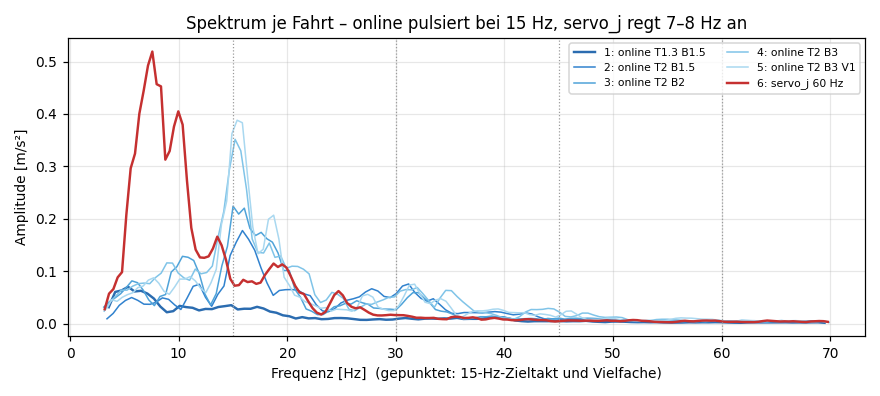
\includegraphics[width=\textwidth]{m4/03_handy_spektrum.png}
  \caption[Spektrum der Beschleunigung am Unterarm]{Spektrum der Beschleunigung am Unterarm
  je Fahrt. Rot: \code{servo_j} mit \SI{60}{\hertz}; blau: Varianten mit Interpolation in der
  Steuerung (\code{movelinear_online}).}
  \label{fig:spektrum}
\end{figure}

\paragraph{Untersuchte Lösungen.} \Cref{tab:zittern} fasst die Wege zusammen.
\begin{table}[htbp]
  \centering
  \caption{Untersuchte Ausführungsarten gegen das Zittern}
  \label{tab:zittern}
  \small
  \begin{tabularx}{\textwidth}{@{}>{\raggedright\arraybackslash}p{36mm} X X@{}}
    \toprule
    Ausführungsart & Vorteil & Nachteil \\
    \midrule
    höhere Rate von \code{servo_j} & kleinere Stufen & Laptop schafft sie über NeuraPy
      nicht stabil \\
    Bahnpuffer der Steuerung & Steuerung fährt glatt & in der vorhandenen Version nicht
      verfügbar \\
    \code{movelinear_online} (Steuerung interpoliert, 15 Ziele/s) & Schwingung
      \SI{-76}{\percent} & in Drehungen bis \SI{49}{\milli\metre} neben der Bahn und bis
      \SI{0.79}{rad} hinterher; kehrte \SI{27}{\milli\metre} über dem Greifpunkt um \\
    \code{servo_j} mit Override \num{0.5} & so ruhig wie ein Herstellerprogramm, Bahn
      $\le$ \SI{1.2}{\milli\metre} & Steuerung folgt etwa \SI{0.09}{\second} verzögert \\
    \bottomrule
  \end{tabularx}
\end{table}

\paragraph{Entscheidung.} Zunächst wurde \code{movelinear_online} gewählt, weil es die
Schwingung am stärksten senkte. Die Nachrechnung zeigte aber, dass der Arm damit in Kurven so
weit hinter der Sollbahn lag, dass die Schleppfehlerprüfung der Aufnahme und die
Sicherheitsprüfung der Ausführung jede Fahrt abgebrochen hätten. Für die Datenpaare ist das
grundsätzlich: Zustand und Sollstellung müssen zueinander passen. Am Labortag vom 19.10.\
bestätigte sich die Alternative: Mit \code{servo_j} und Override \num{0.5} führt die
Steuerung die Sollwerte weicher nach. Die Schwingung lag bei
\SIrange{0.19}{0.20}{\metre\per\second\squared} statt \SI{1.74}{\metre\per\second\squared}, also
auf dem Niveau eines Programms am Bedienhandgerät
(\SIrange{0.16}{0.18}{\metre\per\second\squared}, \cref{fig:h1}). Die Bahn wich höchstens
\SI{1.2}{\milli\metre} ab, und die Fahrzeit blieb gleich. Seitdem gilt \code{servo_j} mit
Override \num{0.5} für Aufnahme und Ausführung.

\begin{figure}[htbp]
  \centering
  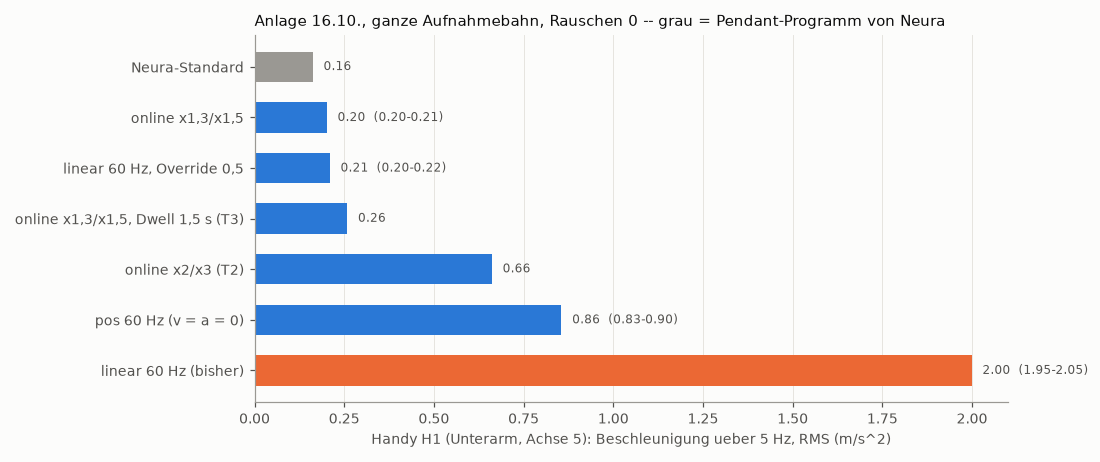
\includegraphics[width=\textwidth]{m4/13_labortag16_h1.png}
  \caption[Schwingung am Unterarm je Ausführungsart]{Schwingung am Unterarm über die ganze
  Aufnahmebahn je Ausführungsart (Effektivwert oberhalb \SI{5}{\hertz}, ohne Rauschen). Grau:
  Programm am Bedienhandgerät zum Vergleich.}
  \label{fig:h1}
\end{figure}

\todo[inline]{Override \num{0.5} mit dem Betreuer abstimmen und hier vermerken.}

Die ausführliche Untersuchung mit allen Messreihen steht in
\code{Dokumentation/Zittern-an-der-Anlage.md}; die Rohdaten liegen unter \code{Berichte/}.

% ==============================================================================
\section{Erfolgs- und Abbruchkriterium}
\label{sec:erfolg}

Die Fahrt gilt als erfolgreich beendet, wenn die Gelenke fünf Takte lang höchstens
\SI{0.02}{rad} von der Endstellung der Aufnahme entfernt sind und der Greifer geschlossen ist,
frühestens nach der halben typischen Episodenlänge. Die Stellung allein reicht nicht: In der
Simulation lag ein Zwischenpunkt auf dem Weg an derselben Stelle wie der Endpunkt, und ohne
Greiferbedingung wurde eine Fahrt mitten in der Bahn als fertig gewertet.

Früher wurde zusätzlich der Abstand zum Greifpunkt der Aufnahme bewertet. Bei wechselnden
Objektlagen ist das nicht mehr sinnvoll; dieser Wert ist nur noch Information. Abgebrochen
wird nach dem \num{1.5}-Fachen der längsten Episode, bei verletzter Sicherheitsprüfung
(\cref{ch:sicherheit}) oder wenn keine Vorhersage mehr rechtzeitig vorliegt.

Für Versuche mit bekannter Objektlage gibt es einen Probegriff: Die Policy fährt selbst, die
Lage ist aber wie bei der Aufnahme bekannt. Ziele, die tiefer als ein einstellbarer Abstand
über dem Bauteil liegen (Standard \SI{25}{\milli\metre}), werden abgelehnt. So lässt sich
prüfen, wohin die Policy greifen würde, ohne dass sie auf das Bauteil oder den Tisch fährt.

\paragraph{Protokoll.} Jede Fahrt wird mit allen Takten gespeichert: Zustand, Sollwerte, rohe
Vorhersagen, Vorhersagezeit, Verzug der Folgen, gekappte Takte und Abbruchgrund. Eine
Live-Ansicht zeigt während der Fahrt die Kamerabilder, die Spur des \ac{tcp} und die gerade
gemittelten Vorhersagen.

\chapter{Sicherheitskonzept}
\label{ch:sicherheit}

% ==============================================================================
\section{Gefährdungen durch eine gelernte Policy}
\label{sec:gefahren}

Eine programmierte Bahn lässt sich vor der Fahrt vollständig prüfen. Bei einer gelernten
Policy ist das nicht möglich: Sie erzeugt ihre Sollwerte erst während der Fahrt, und in
Zuständen außerhalb der Trainingsdaten ist ihr Verhalten nicht vorhersagbar
(\cref{sec:covariate-shift}). Typische Fehlbilder aus den Versuchen sind ein Abtauchen in
Richtung Tisch, Sprünge zwischen zwei Vorhersagen und ein Stehenbleiben an Haltepunkten.
Hinzu kommen technische Fehler wie ein eingefrorenes Kamerabild oder ein unterbrochener
Steuerkanal.

NeuraPy bietet keine frei definierbaren Schutzräume. Modul~4 baut deshalb eine eigene,
mehrstufige Sicherheitsschicht zusätzlich zu den Schutzfunktionen des Roboters
(\cref{fig:sicherheit}). Der Hardware-Not-Halt bleibt bei allen Fahrten in Reichweite; ein
Software-Stopp ersetzt ihn nicht.

\begin{figure}[htbp]
  \centering
  \begin{tikzpicture}[font=\small, node distance=3.5mm,
      st/.style={draw, rounded corners=1.5mm, align=left, text width=96mm, minimum height=9mm,
                 inner xsep=3mm},
      tag/.style={font=\scriptsize\bfseries, anchor=east, align=right, text width=26mm},
      arr/.style={-{Stealth[length=2mm]}, thick}]
    \node[st, fill=blue!6] (s1) {Weiche Begrenzung: Änderung je Takt $\le$ \SI{0.8}{rad/s}, Richtung bleibt};
    \node[st, fill=blue!10, below=of s1] (s2) {Zielprüfung: Ziel und Nachlauf gegen Tisch, Sperrzonen,
      Hindernisse und Hülle der Demonstrationen};
    \node[st, fill=blue!14, below=of s2] (s3) {Harte Grenze je \SI{60}{\hertz}-Sollwert: endlich, Achsgrenzen,
      $\le$ \SI{1.0}{rad/s}, Ziel--Ist $\le$ \SI{0.35}{rad}};
    \node[st, fill=orange!12, below=of s3] (s4) {Überwachung (eigener Thread, \SI{20}{\hertz}): gemessene
      Stellung gegen Kollisionsmodell};
    \node[st, fill=orange!16, below=of s4] (s5) {Bildalter, stehender Arm, Vorhersage zu spät};
    \node[st, fill=red!10, below=of s5] (s6) {Schutzfunktionen der Steuerung, Hardware-Not-Halt};
    \node[tag] at ([xshift=-2mm]s1.west) {vor dem Senden};
    \node[tag] at ([xshift=-2mm]s4.west) {während der Fahrt};
    \node[tag] at ([xshift=-2mm]s6.west) {Anlage};
    \draw[arr] ([xshift=4mm]s1.east) -- ([xshift=4mm]s6.east)
      node[midway, right, font=\scriptsize, align=left] {letzte\\Instanz};
  \end{tikzpicture}
  \caption[Stufen der Sicherheitsschicht]{Stufen der Sicherheitsschicht von Modul~4. Die
  oberen Stufen prüfen jeden Befehl, bevor er die Steuerung erreicht, die unteren den
  tatsächlichen Zustand während der Fahrt.}
  \label{fig:sicherheit}
\end{figure}

% ==============================================================================
\section{Prüfung vor dem Senden}
\label{sec:pruefung-senden}

\paragraph{Weiche Begrenzung.} Die Änderung der Sollstellung je Takt wird auf eine
Gelenkgeschwindigkeit von \SI{0.8}{rad/s} begrenzt; die Richtung bleibt erhalten.
\emph{Begründung:} Die Daten enthalten Korrekturen bis etwa \SI{1}{rad/s}, und beim
Eintreffen einer verspäteten Vorhersage springt der Mittelwert kurzzeitig. Ohne diese Stufe
stoppte die harte Grenze eine sonst gute Fahrt bei \SI{1.03}{rad/s}.

\paragraph{Zielprüfung.} Jedes Ziel der Policy wird vor dem Senden gegen das Kollisionsmodell
geprüft. Dazu werden aus den Gelenkwinkeln die Positionen von Werkzeug, Kamera, Handgelenk und
Ellbogen berechnet und mit Tisch, Sperrzonen und festen Hindernissen verglichen. Der Tisch
wird live aus den Tischpunkten der Steuerung gelesen, ersatzweise aus den Werten der Aufnahme.
Zusätzlich muss das Werkzeug innerhalb der um \SI{3}{\centi\metre} erweiterten Hülle aller
Demonstrationen bleiben.

\begin{description}
  \item[Problem] Zuerst prüfte nur die Überwachung die \emph{gemessene} Stellung. Sie reagiert
    erst, wenn der Arm schon an der Grenze ist; mit Prüftakt und Stoppzeit kommt der Stopp
    einige Millimeter zu spät. Und nach einem abgelehnten Ziel lief der Arm an der Anlage noch
    bis zu \SI{7.5}{\milli\metre} nach.
  \item[Lösung] Geprüft wird das Ziel selbst, und zusätzlich das um einen Takt linear
    verlängerte Ziel. So wird bereits abgelehnt, solange der Nachlauf bei der aktuellen
    Geschwindigkeit noch vor der Grenze endet.
\end{description}

\paragraph{Harte Grenze.} Jeder einzelne \SI{60}{\hertz}-Sollwert wird im Adapter verworfen,
wenn er nicht endlich ist, außerhalb der Achsgrenzen liegt oder eine Gelenkgeschwindigkeit
über \SI{1.0}{rad/s} gegenüber dem letzten Sollwert erfordert. Die Zeitbasis dafür ist nach
unten begrenzt, ein Stocken des Takts erlaubt also keinen großen Sprung. Liegt die
Sollstellung mehr als \SI{0.35}{rad} von der gemessenen entfernt, wird ebenfalls nichts
gesendet. In allen Fällen stoppt der Roboter. Diese Grenze gilt auch bei Aufnahme und Teachen.

% ==============================================================================
\section{Überwachung während der Fahrt}
\label{sec:ueberwachung}

\begin{description}
  \item[Arbeitsraum] Ein eigener Thread prüft alle \SI{50}{\milli\second} die gemessene
    Stellung gegen dasselbe Kollisionsmodell. Er läuft getrennt von der Vorhersage, damit eine
    verzögerte Vorhersage den Stopp nicht verzögert.
  \item[Eingefrorenes Bild] Ist ein Kamerabild zwei Takte in Folge älter als
    \SI{100}{\milli\second}, hält die Fahrt an. Die Policy würde sonst auf ein veraltetes Bild
    reagieren, ohne es zu merken.
  \item[Stehender Arm] Bewegt sich der Arm fünf Takte lang praktisch nicht, obwohl das Ziel
    mehr als \SI{0.02}{rad} entfernt ist, endet die Fahrt. \emph{Anlass:} Der Not-Halt am
    Bedienhandgerät hält den Arm an, ohne dass \code{servo_j} einen Fehler meldet. Die Fahrt
    schickte weiter Ziele, und nach dem Entriegeln hätte ein weit entferntes Ziel angelegen.
  \item[Vorhersage zu spät] Liegt keine gültige Vorhersage mehr für den aktuellen Takt vor,
    endet die Fahrt (\cref{sec:takt}).
\end{description}

% ==============================================================================
\section{Stoppverhalten und Freigabe}
\label{sec:stopp}

Der Software-Stopp hielt den Arm an der Anlage innerhalb von \SI{96}{\milli\second} an. Der
Befehl zum Beenden der Online-Bewegung bremst dagegen nicht, er wird deshalb für Abbrüche
nicht verwendet. Fahrten am realen Roboter erfordern eine ausdrückliche Bestätigung; aus dem
Ablauf des Gesamtsystems wird die Freigabe des dortigen Sicherheitsdialogs übernommen
(\cref{ch:integration}).

\paragraph{Grenzen.} Die Sicherheitsschicht erkennt, was sich im Kollisionsmodell abbilden
lässt. Ein Greifen neben das Bauteil oder ein Anstoßen des Bauteils innerhalb des erlaubten
Raums verhindert sie nicht. Die Grenzwerte der Gelenkgeschwindigkeiten stammen aus Daten der
\ac{vm} und wurden an der Anlage bestätigt; die Achsgrenzen stammen aus dem \ac{urdf}.

\todo[inline]{Achsgrenzen gegen Datenblatt bzw.\ Bedienhandgerät abgleichen (im Code noch als
nicht verifiziert markiert).}

\chapter{Einbindung in das Gesamtsystem}
\label{ch:integration}

Modul~4 wurde zunächst in einem eigenen Repository entwickelt und anschließend in das
Repository der Gruppe übernommen \quelle{INTEGRATION.md}. Dort ist es auf zwei Wegen
erreichbar: als Greifvariante im automatischen Ablauf und als eigener Reiter in der
gemeinsamen Bedienoberfläche.

% ==============================================================================
\section{Schnittstelle zum Ablauf}
\label{sec:grasper}

Der Ablauf des Gesamtsystems ist ein Zustandsautomat, in dem das Greifen über eine
Schnittstelle \code{Grasper} angesprochen wird. Die Variante von Modul~4 übernimmt nur den
Zustand PICK; das Ablegen auf der Prüfvorrichtung macht weiterhin Modul~2.

\paragraph{Eigene Python-Umgebung.} LeRobot~0.6.1 setzt Python~3.12 voraus, und seine
Abhängigkeiten kollidieren mit denen der Texterkennung von Modul~3. Die Policy läuft deshalb
als Unterprozess in einer eigenen Umgebung. Die Bedienoberfläche und die übrigen Module
bleiben in ihrer Umgebung. Der Nachteil ist eine Startzeit von einigen Sekunden je Fahrt; der
Vorteil, dass keine der beiden Umgebungen auf Kompromissversionen festgelegt werden muss.

\paragraph{Ablauf eines Greifvorgangs} (\cref{fig:grasper}):
\begin{enumerate}
  \item Modul~1 gibt die Draufsichtkamera frei, damit Modul~4 sie öffnen kann; Modul~2 trennt
    seine Verbindung zur Steuerung. Je Kamera und je Steuerung darf immer nur ein Prozess
    verbunden sein.
  \item Der Unterprozess startet die Policy und fährt den Roboter. Die Lage aus der
    Objekterkennung wird übergeben, aber nur protokolliert; die Policy findet das Bauteil
    selbst in den Bildern.
  \item Der Fortschritt wird aus der Ausgabe des Unterprozesses gelesen. Erreicht die Policy
    den Übergabepunkt nicht oder dauert die Fahrt länger als \SI{300}{\second}, gilt das
    Greifen als fehlgeschlagen, und der Ablauf geht in den Fehlerzustand.
  \item Für das Ablegen verbindet sich Modul~2 wieder, setzt Werkzeug, Override und
    Bewegungsprogramm auf seine eigenen Werte zurück und legt das Bauteil ab.
\end{enumerate}

\begin{figure}[htbp]
  \centering
  \begin{tikzpicture}[font=\small, x=1cm, y=1cm]
    \foreach \x/\n in {0/Ablauf, 3.4/Modul~1, 6.8/{Modul~4\\(Unterprozess)}, 10.2/Modul~2} {
      \node[draw, rounded corners=1.5mm, fill=black!5, text width=24mm, align=center,
            minimum height=9mm, font=\scriptsize] at (\x,0) {\n};
      \draw[black!30, densely dashed] (\x,-0.45) -- (\x,-6.3);
    }
    \def\msg#1#2#3#4{\draw[-{Stealth[length=2mm]}, thick] (#1,#3) -- node[above, font=\scriptsize, fill=white, inner sep=1pt] {#4} (#2,#3);}
    \msg{0}{3.4}{-1.0}{Lage bestimmen, Kamera freigeben}
    \msg{0}{10.2}{-1.7}{Verbindung trennen}
    \msg{0}{6.8}{-2.4}{Policy starten (Lage nur Protokoll)}
    \fill[blue!10] (6.55,-2.6) rectangle (7.05,-4.4);
    \node[font=\scriptsize, anchor=west, align=left] at (7.15,-3.5) {greifen, fahren\\bis PRE\_PLACE};
    \draw[-{Stealth[length=2mm]}, thick, densely dashed] (6.8,-4.6) -- node[above, font=\scriptsize] {Übergabepunkt erreicht} (0,-4.6);
    \msg{0}{10.2}{-5.4}{verbinden, Einstellungen zurücksetzen, ablegen}
  \end{tikzpicture}
  \caption[Ablauf eines Greifvorgangs mit Modul~4]{Ablauf eines Greifvorgangs mit Modul~4
  im Gesamtsystem (vereinfacht).}
  \label{fig:grasper}
\end{figure}

\todo[inline]{Höhe des Übergabepunkts über der Prüfvorrichtung vereinheitlichen: Hindernismodell
nennt \SI{7}{\centi\metre}, Orchestrator etwa \SI{9}{\centi\metre}.}

% ==============================================================================
\section{Bedienoberfläche}
\label{sec:gui}

Die Bedienoberfläche von Modul~4 ist als Reiter in die gemeinsame Oberfläche eingebunden und
lässt sich auch eigenständig starten; es ist dieselbe Oberfläche. Sie gliedert sich in vier
Bereiche:
\begin{description}
  \item[Systemcheck] Prüfung von Umgebung, Grafikkarte, Kameras, Verbindung zur Steuerung,
    Kinematik und Sollwerttakt; die Ergebnisse werden als Bericht gespeichert.
  \item[Aufnahme] Ablauftabelle mit Teachen und Touch-up, Tischpunkte, Kameraeinstellungen,
    Einstellungen für Rauschen, Versatz und Objektlagen, Start der Aufnahme und Abdeckungskarte
    der bisherigen Lagen.
  \item[Training] Export und Training mit Fortschrittsanzeige.
  \item[Betrieb] Auswahl eines Modells, Fahrten mit Live-Ansicht, Probegriff bei bekannter
    Lage.
\end{description}
Dass immer nur eine Seite den Roboter und die Draufsichtkamera benutzt, regelt die gemeinsame
Oberfläche. Die Bedienung im Einzelnen beschreibt die Bedienanleitung (Dokument~C).

\chapter{Versuche und Ergebnisse}
\label{ch:versuche}

Dieses Kapitel fasst die Versuche in zeitlicher Reihenfolge zusammen. Zu jedem Versuch gibt
es im Ordner \code{Berichte/} ein Testprotokoll mit Rohdaten und Auswerteskripten;
\cref{app:berichte} listet sie auf. Die Versuche bauen aufeinander auf: Jeder Befund hat die
Fragestellung des nächsten bestimmt.

% ==============================================================================
\section{Testumgebungen und Kennzahlen}
\label{sec:kennzahlen}

Versuche liefen in drei Umgebungen, die unterschiedlich aussagekräftig sind
(\cref{tab:umgebungen}). Ein Versuch in der \ac{vm} oder offline ist \emph{keine}
Anlagenmessung; in den Protokollen ist das bei jeder Fahrt über die Kennung der Steuerung
festgehalten. Die wichtigsten Kennzahlen sind:

\begin{description}
  \item[Nächste Annäherung] kleinster waagerechter Abstand des \ac{tcp} zum Greifpunkt rund um
    das Schließen des Greifers; Median und Anteil der Fahrten innerhalb \SI{10}{\milli\metre}.
  \item[Greifpunkt beim Schließen] waagerechter Abstand im Takt des Schließbefehls.
  \item[Unter Tisch] Anteil der Fahrten, in denen die Werkzeugspitze unter die Tischfläche
    geht (nur \ac{vm}, dort gibt es keinen echten Tisch).
  \item[Abbruch der harten Grenze] Anteil der Fahrten, die die Sollwertprüfung aus
    \cref{sec:pruefung-senden} beendet hat.
  \item[Endstellung] Anteil der Fahrten, die den Übergabepunkt erreichen.
\end{description}

% ==============================================================================
\section{Vorstudie: Nutzen des eingespeisten Rauschens}
\label{sec:rauschstudie}

\paragraph{Frage.} Lohnt sich das Rauschen, und welche Form ist die beste? Die Frage musste vor
der ersten Aufnahme beantwortet werden, als noch keine Anlage und keine Bilder verfügbar waren.

\paragraph{Vorgehen.} Mit derselben Planungs- und Rauschkette wurde ein einfaches Netz ohne
Bilder trainiert und in der eigenen Simulation mit verschobenen Objektlagen und seitlichen
Stößen von \SI{15}{\milli\metre} geprüft, je Variante fünf Trainingsläufe mit je 24
Objektlagen \quelle{Berichte/2026-09-16_Rauschstudie.pdf}.

\begin{table}[htbp]
  \centering
  \caption[Ergebnis der Rauschstudie]{Ergebnis der Rauschstudie (ohne Bilder). Erfolg:
  Greifen weniger als \SI{5}{\milli\metre} neben dem Greifpunkt und Übergabe mit geschlossenem
  Greifer.}
  \label{tab:rauschstudie}
  \begin{tabularx}{\textwidth}{@{}X r r r@{}}
    \toprule
    Rauschen & ungestört & mit Stößen & Greiffehler \\
    \midrule
    ohne & \SI{32}{\percent} & \SI{12}{\percent} & \SI{3.4}{\milli\metre} \\
    fest, \SI{15}{\milli\metre} / \ang{2.9} & \SI{90}{\percent} & \SI{92}{\percent} & \SI{0.6}{\milli\metre} \\
    je Episode zufällig, 0--\SI{15}{\milli\metre} / 0--\ang{2.9} & \SI{92}{\percent} & \SI{93}{\percent} & \SI{0.5}{\milli\metre} \\
    \bottomrule
  \end{tabularx}
\end{table}

\paragraph{Ergebnis.} Ohne Rauschen gelang ein Drittel der Fahrten, mit Rauschen rund neun von
zehn (\cref{tab:rauschstudie}). Die zufällige Stärke je Episode war bei Stößen am besten und
erzeugte die ruhigsten Bewegungen; sie wurde übernommen. Weil die Studie ohne Bilder und mit
einem anderen Netz arbeitet, ist das Ergebnis nur der Tendenz nach übertragbar.

% ==============================================================================
\section{Durchstich in Simulation und VM}
\label{sec:durchstich}

\paragraph{Frage.} Läuft die ganze Kette aus Aufnahme, Export, Training und Ausführung, und
passen Zustand und Aktion zusammen?

\paragraph{Vorgehen.} Aufnahme und Ausführung in der eigenen Simulation und in der \ac{vm}, mit
Platzhalterbildern ohne Bezug zur Szene. Die Policy konnte also nur aus dem Zustand lernen
\quelle{Berichte/2026-09-17_Durchstich_Policy.pdf}.

\begin{table}[htbp]
  \centering
  \caption[Durchstich mit Platzhalterbildern]{Durchstich mit Platzhalterbildern. Werte als
  Median über die Fahrten.}
  \label{tab:durchstich}
  \begin{tabularx}{\textwidth}{@{}X r r r r@{}}
    \toprule
    Umgebung (Datensatz) & Erfolg & Greifpunkt & Bahn p95 & Vorhersage \\
    \midrule
    Simulation (50 Episoden) & 10/10 & \SI{1.6}{\milli\metre} & \SI{4.0}{\milli\metre} & \SI{117}{\milli\second} \\
    \acs{vm} (30 Episoden) & 0/5 & -- & \SI{5.2}{\milli\metre} & \SI{85}{\milli\second} \\
    \bottomrule
  \end{tabularx}
\end{table}

\paragraph{Ergebnis.} In der Simulation fuhr die Policy alle zehn Fahrten selbst
(\cref{tab:durchstich,fig:durchstich}). In der \ac{vm} folgte sie der Bahn bis zur
Vorgreifposition und blieb dort in allen Fahrten stehen: Eine Gelenkfahrt endete im Stillstand,
die folgende Linearfahrt begann aus dem Stillstand, und im Zustand war beides nicht zu
unterscheiden (\cref{sec:multimodal}). Daraus entstand das Überschleifen an
Durchfahrpunkten (\cref{sec:bahnplanung}). Der Durchstich zeigte außerdem den Bildzähler als
ungewollte Zeitinformation (\cref{sec:validierung}) und die gezackten Folgen bei
Rauschvorhersage (\cref{sec:netz}).

\begin{figure}[htbp]
  \centering
  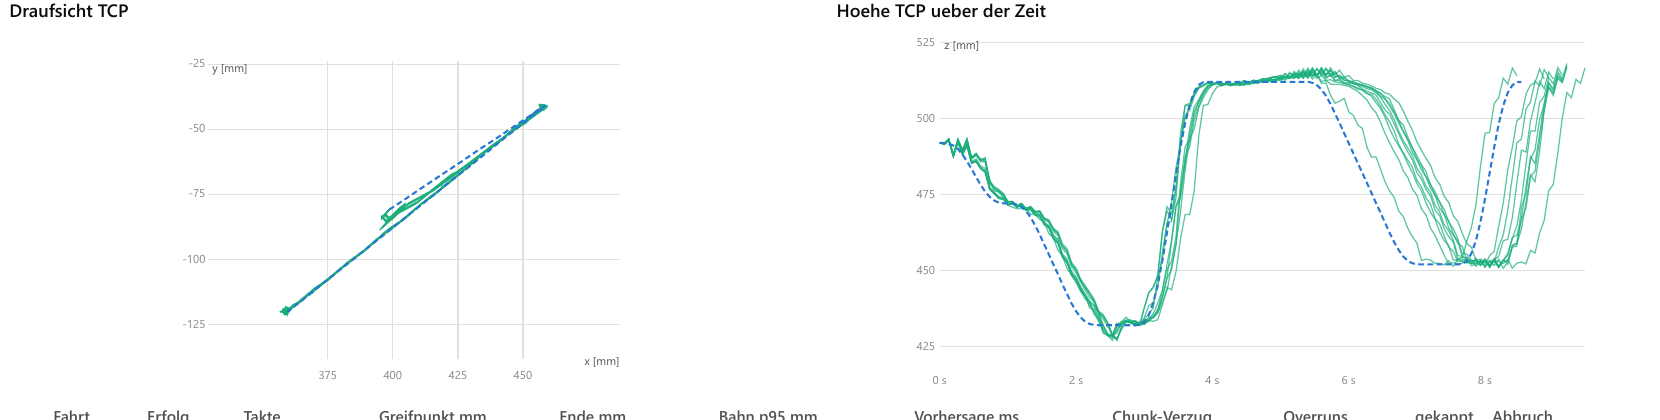
\includegraphics[width=\textwidth]{m4/durchstich_sim_rollouts.png}
  \caption[Fahrten der Policy im Durchstich in der Simulation]{Zehn Fahrten der Policy in
  der Simulation: Draufsicht (links) und Höhe des \acs{tcp} über der Zeit (rechts). Blau
  gestrichelt die ideale Bahn der Aufnahme, grün die Fahrten der Policy.}
  \label{fig:durchstich}
\end{figure}

% ==============================================================================
\section{Inbetriebnahme an der Anlage}
\label{sec:labortage}

An mehreren Labortagen zwischen dem 01.10.\ und dem 21.10.\ wurden die Adapter nach der
Abnahmeliste aus \cref{sec:testkonzept} geprüft. Die wichtigsten Befunde sind bereits in den
jeweiligen Kapiteln beschrieben:
\begin{itemize}
  \item Kinematik der Anlage identisch mit der \ac{vm} (\cref{sec:kinematik}),
  \item abbrechende Bahnen durch einen gedrosselten Rechner und Schleppfehler durch einen zu
    kleinen Override (\cref{sec:sollwerte}),
  \item Zittern bei \code{servo_j} und die Entscheidung für Override \num{0.5}
    (\cref{sec:zittern}),
  \item Kameras nur mit voller Bildrate direkt am Rechner, nicht an einem Verteiler
    (\cref{sec:kameras}).
\end{itemize}
Sechs Aufnahme-Episoden mit der endgültigen Ausführungsart liefen ohne Abbruch; der Arm lag
höchstens \SIrange{0.06}{0.10}{rad} hinter der Sollstellung und damit weit innerhalb der
Grenzen.

% ==============================================================================
\section{Datensätze}
\label{sec:datensaetze}

Ab Ende Oktober wurden an der Anlage Demonstrationen mit echten Bildern aufgenommen
(\cref{tab:datensaetze}). Alle Aufnahmen verwenden \code{servo_j} mit Override \num{0.5},
\SI{15}{\hertz}, beide Kameras und den Transfer mit \SI{0.15}{\metre\per\second}; der Endanflug
lag bis zum 17.11.\ bei \SI{0.05}{\metre\per\second}. Licht (Decke an oder aus, Tageslicht)
und Lage der Draufsichtkamera wurden zwischen den Sitzungen bewusst variiert.

\begin{table}[htbp]
  \centering
  \caption{Aufgenommene Datensätze an der Anlage}
  \label{tab:datensaetze}
  \small
  \begin{tabularx}{\textwidth}{@{}l r X@{}}
    \toprule
    Datensatz & Episoden & Bemerkung \\
    \midrule
    26.10. & 167 & erstes Modell mit echten Bildern \\
    02., 03.\ und 09.11. & 602 & Grundlage der meisten Modelle (\SI{82591}{} Takte, ein Bauteil,
      164 Lagen) \\
    11.11. & 151 & 50 Lagen; 20 davon als feste Testlagen zurückgehalten \\
    ab 19.11. & -- & neuer Datensatz nach den Standards aus \cref{sec:folgerungen} \\
    \bottomrule
  \end{tabularx}
\end{table}

% ==============================================================================
\section{Modellprüfung des Checkpoints vom 09.11.}
\label{sec:modellpruefung}

\paragraph{Frage.} Lernt das Modell auf 602 Episoden, und findet es unbekannte Lagen?

\paragraph{Vorgehen.} Training mit \num{10000} Schritten, Batchgröße 128, in \SI{77}{\minute}.
Danach Stufe~2 in der \ac{vm} (\cref{sec:replay}) an acht unbekannten und drei bekannten Lagen
\quelle{Berichte/2026-11-10_Modellpruefung_Checkpoint_2026-11-09.pdf}.

\paragraph{Ergebnis.}
\begin{itemize}
  \item Der Validierungsverlust sank bis zum Schluss ohne Anzeichen von Überanpassung und lag
    rund fünfmal niedriger als beim Modell vom 26.10. Der mittlere Gelenkfehler betrug
    \SI{0.008}{rad}.
  \item Die offline gemessene Genauigkeit sagt wenig über neue Lagen: Nahe am Greifpunkt
    verrät der Zustand das Ziel bereits, die Bilder werden dort kaum gebraucht.
  \item In der \ac{vm} trafen unbekannte Lagen in der Mitte des Arbeitsraums den Greifpunkt
    auf \SIrange{5}{22}{\milli\metre}, im Median \SI{15}{\milli\metre}. Am fernen Rand
    ($x > \SI{0.5}{\metre}$) gab es reproduzierbare Fehlgriffe um \SIrange{7}{10}{\centi\metre}.
  \item Für Bauteile mit \ang{0} bis \ang{90} Drehung waren die Demonstrationen zur Hälfte um
    \ang{180} gedreht gegriffen; der Griff ist mehrdeutig (\cref{sec:multimodal}).
  \item 6 von 15 Fahrten gingen unter die Tischfläche, bis \SI{56}{\milli\metre}. Der damalige
    Arbeitsraumschutz lag pauschal \SI{145}{\milli\metre} unter dem Tisch und hätte keine davon
    gestoppt. Daraufhin wurde der Tisch aus den Tischpunkten in das Kollisionsmodell und in die
    Modellbeschreibung aufgenommen (\cref{sec:tisch,sec:pruefung-senden}).
\end{itemize}

\begin{figure}[htbp]
  \centering
  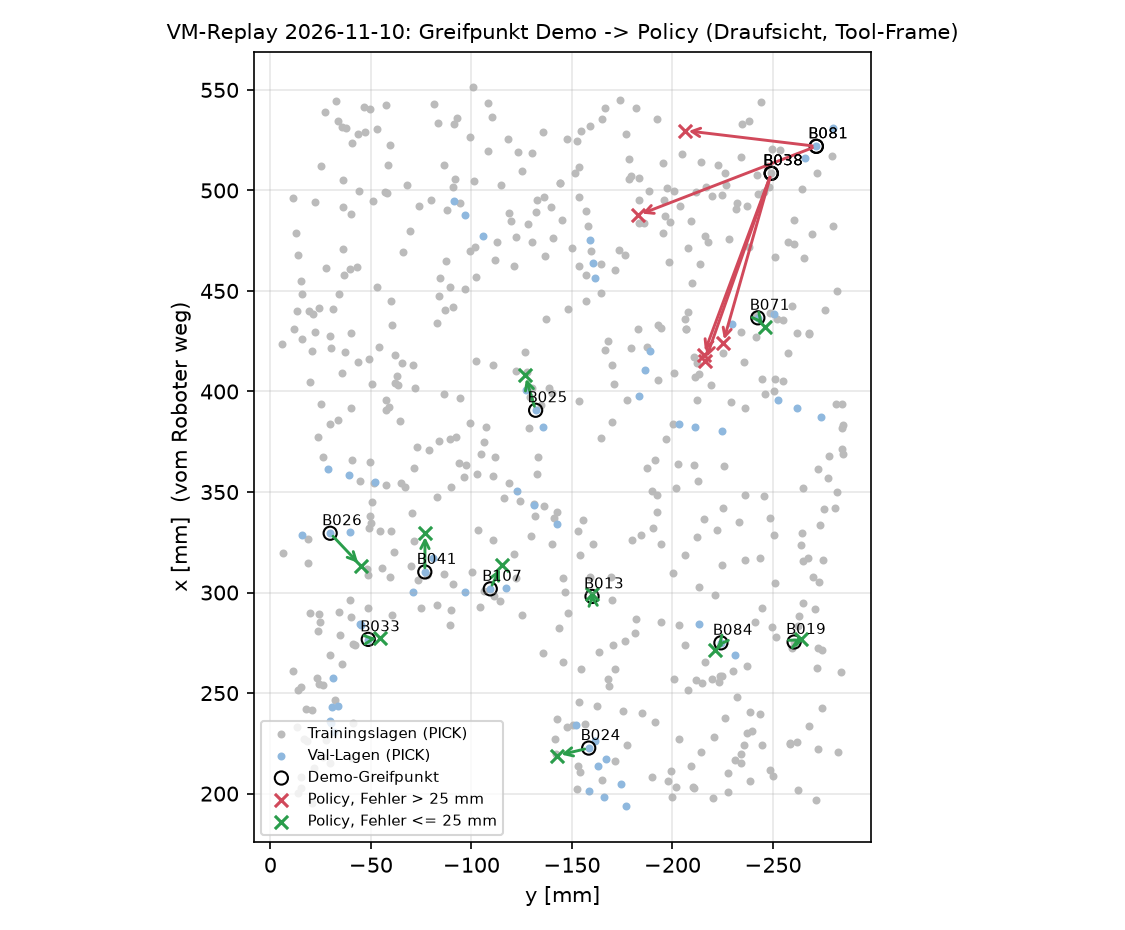
\includegraphics[width=0.85\textwidth]{versuche/modellpruefung_greifpunkte.png}
  \caption[Greifpunkte in der Modellprüfung vom 10.11.]{Greifpunkte der Policy in der
  Modellprüfung vom 10.11.\ (\acs{vm}, Bilder der Aufnahme) gegenüber den Greifpunkten der
  Demonstrationen.}
  \label{fig:modellpruefung}
\end{figure}

% ==============================================================================
\section{VM-Test mit den Aufnahmen vom 11.11.}
\label{sec:replay-1111}

\paragraph{Frage.} Wie verhält sich das Modell an einem Tag, den es nie gesehen hat, und wie
oft würde es in den Tisch fahren?

\paragraph{Vorgehen.} Stufe~1 und Stufe~2 mit allen 151 Episoden vom 11.11.\
\quelle{Berichte/2026-11-13_VM-Replay_Daten-2026-11-11.pdf}.

\paragraph{Ergebnis.} Offline lag der Gelenkfehler je Takt im Median bei \ang{0.7} bis
\ang{1.8}; die Policy ist glatt und genau, wenn Bild und Zustand zusammenpassen. In der \ac{vm}
lag die nächste Annäherung im Median bei \SI{10.7}{\milli\metre}, \SI{49}{\percent} der
Fahrten innerhalb \SI{10}{\milli\metre}, \SI{90}{\percent} innerhalb \SI{39}{\milli\metre}
(\cref{fig:replay-1111}). Ein neuer Tag war damit nicht schlechter als ein Trainingstag, und ein
Unterschied zwischen Licht an und aus war nicht nachweisbar. Zwei Probleme blieben:
\begin{itemize}
  \item In 81 von 151 Fahrten ging die Werkzeugspitze unter die Tischfläche, meist kurz
    \emph{nach} dem Schließen beim seitlichen Wegfahren. Eine Gegenprobe mit Bildwahl nach
    Position statt nach Takt ergab dasselbe; es ist also kein reines Testartefakt.
  \item 22 Fahrten wurden im Transport von der harten Grenze abgebrochen.
\end{itemize}
Die Schwingbahnen in der \ac{vm} stammen überwiegend aus dem Testverfahren selbst: Die
Bilder zeigen die verrauschte Bahn der Aufnahme, der Arm ist aber woanders, und die Policy
korrigiert Abweichungen, die es nicht gibt.

\begin{figure}[htbp]
  \centering
  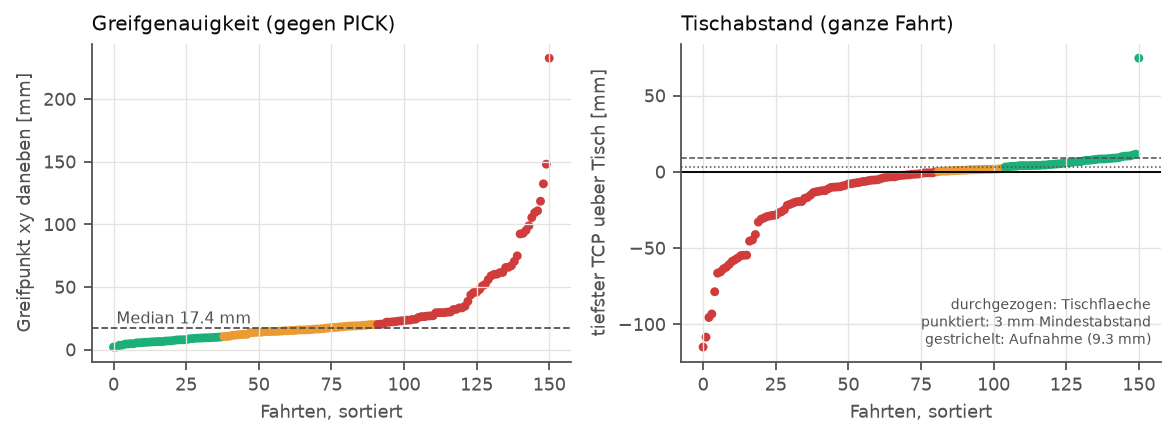
\includegraphics[width=\textwidth]{versuche/replay_fehler_tisch.png}
  \caption[VM-Test mit den Aufnahmen vom 11.11.]{VM-Test mit den Aufnahmen vom 11.11.\
  (151 Fahrten, sortiert). Links der waagerechte Abstand zum Greifpunkt beim Schließen, rechts
  der tiefste Punkt des \acs{tcp} über der Tischfläche.}
  \label{fig:replay-1111}
\end{figure}

% ==============================================================================
\section{Versuchsreihe Policy-Varianten}
\label{sec:varianten}

\paragraph{Frage.} Lassen sich die Probleme aus \cref{sec:replay-1111} mit den vorhandenen
Daten beheben? Jede Maßnahme wurde einzeln gemessen
\quelle{Berichte/Versuchsreihe_Policy-Varianten/}.

\paragraph{Vorgehen.} Aus den 50 Lagen vom 11.11.\ wurden 20 als feste Testlagen gewählt und
aus allen Trainingsdaten herausgenommen; getestet wurde mit ihren 59 Episoden in der \ac{vm}.
Jede Variante unterscheidet sich von der Basis~A in genau einer Änderung und wurde mit
\num{10000} Schritten trainiert (\cref{tab:varianten-def}). Ausgewertet wurde paarweise je
Testlage mit Vorzeichentest. Zwei Durchläufe desselben Modells streuten bei Annäherung und
Tisch um etwa \SI{\pm 1.5}{\milli\metre} und \SI{\pm 3}{Prozentpunkte}, bei Abbrüchen und
Endstellung um bis zu \SI{18}{Prozentpunkte}; diese beiden Werte sind nur bei großen
Unterschieden deutbar.

\begin{table}[htbp]
  \centering
  \caption{Varianten der Versuchsreihe}
  \label{tab:varianten-def}
  \small
  \begin{tabularx}{\textwidth}{@{}l X X@{}}
    \toprule
    Variante & Änderung & prüft \\
    \midrule
    I & nur Ausführung: stärkere Gewichtung neuer Folgen, seltenere Neuvorhersage & Mitteln der
      Folgen \\
    A Basis & alle Daten ohne Testlagen (694 Episoden) & Bezugspunkt \\
    B Pause kurz & Stillstand am Greifpunkt von 8 auf 3 Takte gekürzt & Mehrdeutigkeit am
      Greifpunkt \\
    C Nur Griff & Episode endet 3 Takte nach dem Schließen; Transport plant der Planer &
      Aufteilung der Aufgabe \\
    D Eine Drehung & um \ang{180} gedrehte Griffe entfernt (529 Episoden) & mehrdeutige
      Greifdrehung \\
    C$'$ (später C2) & wie C, aber ohne die Daten vom 11.11.\ (602 Episoden) & Effekt der
      Daten vom 11.11. \\
    F & wie A, mit Helligkeits- und Farbaugmentierung & Lichtunterschiede \\
    \bottomrule
  \end{tabularx}
\end{table}

\begin{table}[htbp]
  \centering
  \caption[Ergebnisse der Versuchsreihe in der VM]{Ergebnisse der Versuchsreihe in der
  \acs{vm} (59 Fahrten je Modell, Bilder der Testlagen). \enquote{alt}: Checkpoint vom 09.11.,
  ohne Daten vom 11.11.}
  \label{tab:varianten}
  \small
  \begin{tabular}{@{}l r r r r r r@{}}
    \toprule
    Modell & Annäh. & $\le$\SI{10}{mm} & beim Schließen & unter Tisch & Abbruch & Endst. \\
    \midrule
    alt, Seed 0 & \SI{10.2}{mm} & \SI{50}{\percent} & \SI{18.6}{mm} & \SI{54}{\percent} & \SI{32}{\percent} & \SI{41}{\percent} \\
    alt, Seed 1 & \SI{10.6}{mm} & \SI{50}{\percent} & \SI{18.0}{mm} & \SI{59}{\percent} & \SI{36}{\percent} & \SI{59}{\percent} \\
    A & \SI{15.3}{mm} & \SI{28}{\percent} & \SI{28.4}{mm} & \SI{58}{\percent} & \SI{25}{\percent} & \SI{64}{\percent} \\
    B & \SI{15.6}{mm} & \SI{32}{\percent} & \SI{20.8}{mm} & \SI{46}{\percent} & \SI{29}{\percent} & \SI{59}{\percent} \\
    C & \SI{17.5}{mm} & \SI{20}{\percent} & \SI{23.2}{mm} & \SI{36}{\percent} & \SI{14}{\percent} & \SI{85}{\percent} \\
    D & \SI{16.6}{mm} & \SI{33}{\percent} & \SI{26.8}{mm} & \SI{59}{\percent} & \SI{36}{\percent} & \SI{61}{\percent} \\
    C$'$ & \SI{15.5}{mm} & \SI{32}{\percent} & \SI{18.7}{mm} & \SI{47}{\percent} & \SI{7}{\percent} & \SI{90}{\percent} \\
    F & \SI{14.9}{mm} & \SI{29}{\percent} & \SI{26.9}{mm} & \SI{63}{\percent} & \SI{34}{\percent} & \SI{39}{\percent} \\
    \bottomrule
  \end{tabular}
\end{table}

\paragraph{Ergebnisse.}
\begin{enumerate}
  \item \textbf{Ausführung (I):} Weniger Mitteln machte die Fahrt in fast allen Kennzahlen
    schlechter, unruhiger und tiefer. Die Standardeinstellung blieb.
  \item \textbf{Daten vom 11.11.:} Alle Varianten mit diesen Daten trafen schlechter als der
    alte Checkpoint (A auf 17 von 20 Lagen, $p = 0{,}001$). Ein zweites Training mit anderem
    Startwert zeigte, dass die Streuung zwischen Trainings klein ist. Eine Ursache in den Daten
    wurde nicht gefunden: Bahnform, Rauschen, Synchronisation und Kameralage waren an allen
    Tagen gleich; auffällig war nur deutlich mehr Tageslicht. Auch Licht-Augmentierung (F)
    änderte daran nichts. Die Ursache ist offen.
  \item \textbf{Kurze Pause (B):} weniger Tischfahrten, Genauigkeit unverändert.
  \item \textbf{Nur Griff (C, C$'$):} Den Transport dem Planer zu überlassen, senkt
    Tischfahrten und Abbrüche deutlich und lässt fast alle Fahrten durchlaufen. Ohne die
    Daten vom 11.11.\ (C$'$) ist die Genauigkeit beim Schließen so gut wie beim alten
    Checkpoint; die Abbrüche sinken von \SIrange{32}{36}{\percent} auf \SI{7}{\percent}.
  \item \textbf{Eine Drehung (D):} kein Gewinn, aber 165 Demonstrationen weniger.
\end{enumerate}
C$'$ wurde damit das Modell für den ersten Anlagentest (\enquote{C2}). Seitdem endet die
Aufgabe der Policy mit dem Griff, und der Transport zum Übergabepunkt ist geplant.

\todo[inline]{Die Aufteilung \enquote{Policy greift, Planer transportiert} in
\cref{ch:einleitung,ch:integration} nachziehen, sobald sie für den Betrieb endgültig ist. Der
Aufruf aus dem Ablauf (\texttt{m4\_grasper.py}) nutzt den geplanten Transport noch nicht.}

% ==============================================================================
\section{Anlagentest mit C2}
\label{sec:anlagentest-c2}

\paragraph{Frage.} Wie genau trifft die Policy an der realen Anlage?

\paragraph{Vorgehen.} Probegriff mit bekannter Lage (\cref{sec:erfolg}) an fünf Lagen, neun
Fahrten. Die Policy fuhr selbst an und wurde kurz über dem Bauteil angehalten; aus dem Rest
ihrer Vorhersage wurde bestimmt, wo sie gegriffen hätte. Danach korrigierte der Planer auf den
Greifpunkt, griff und legte an einer neuen Lage ab
\quelle{Berichte/2026-11-16_Anlagentest_var_C2.pdf}.

\paragraph{Ergebnis.} Der vorhergesagte Greifpunkt lag im Median \SI{8.7}{\milli\metre}
daneben (\SIrange{1.0}{18.0}{\milli\metre}); 5 von 8 Probegriffen lagen innerhalb
\SI{10}{\milli\metre}. Das passt zum \ac{vm}-Test (\SI{10.7}{\milli\metre}). Der Drehfehler
lag meist unter \ang{5}. \Cref{fig:c2-versatz} zeigt, wo der Fehler entsteht: Bis
\code{PRE_PICK} folgt die Policy der senkrechten Bahn auf \SIrange{1}{7}{\milli\metre};
darunter zögert sie und driftet innerhalb weniger Takte \SIrange{10}{29}{\milli\metre} zur
Seite. Genau diese Zustände kommen in den Demonstrationen nicht vor, weil dort der Trichter
das Rauschen auf null gedämpft hat. Das war der Anlass für den gezielten Versatz im Anflug
(\cref{sec:versatz}) und für \ac{dagger} (\cref{ch:fazit}).

\begin{figure}[htbp]
  \centering
  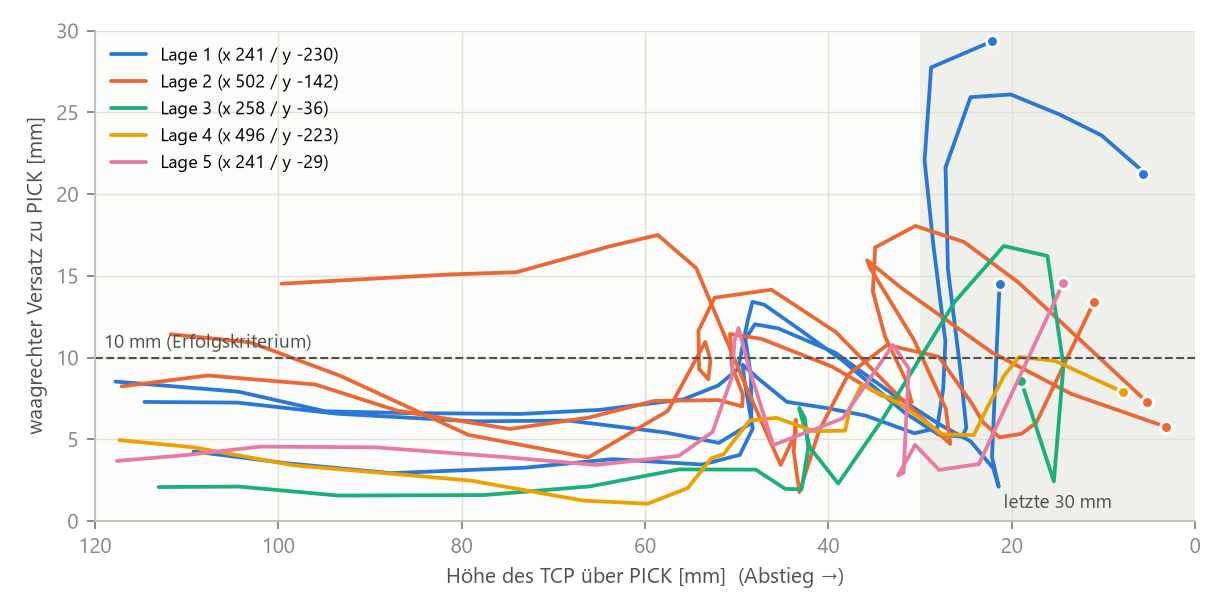
\includegraphics[width=\textwidth]{versuche/c2_versatz_hoehe.png}
  \caption[Seitlicher Versatz über der Höhe im Anlagentest]{Waagerechter Abstand des
  gemessenen \acs{tcp} zum Greifpunkt über der Höhe, je Fahrt im Anlagentest vom 16.11.\
  (Farbe: Lage, Punkt: Stopp).}
  \label{fig:c2-versatz}
\end{figure}

\paragraph{Auffälligkeiten.} Zweimal wurde der Not-Halt am Bedienhandgerät gedrückt, weil der
Arm abzutauchen schien. Die Ausführung bemerkte das nicht und sendete weiter Ziele. Daraus
entstand die Überwachung auf einen stehenden Arm (\cref{sec:ueberwachung}). Ob die Policy
selbst richtig schließt, blieb ungeprüft, weil jede Fahrt vor dem Schließen angehalten wurde.

% ==============================================================================
\section{Empfindlichkeit gegenüber der Kameralage}
\label{sec:kamera-empfindlichkeit}

\paragraph{Frage.} Würde eine Rektifizierung der Draufsicht über die ArUco-Marker helfen?

\paragraph{Vorgehen.} Offline wurden für 30 Episoden (davon 15 von einem Tag, der nicht im
Training war) die Bilder gezielt gestört und die Änderung der Vorhersage gemessen, bei
gleichem Diffusionsrauschen \quelle{Berichte/2026-11-16_Kameraempfindlichkeit_var_C2.pdf}.

\paragraph{Ergebnis} (\cref{fig:kamera}):
\begin{itemize}
  \item Eine Verschiebung der Draufsicht um \SI{10}{Pixel}, was einem um etwa
    \SI{3}{\centi\metre} verschobenen Bauteil entspricht, ändert die Vorhersage nur um
    \SIrange{0.6}{1.5}{\milli\metre}; eine Drehung um \ang{5} um \SIrange{1.0}{1.7}{\milli\metre}.
    Vermutlich hat der zufällige Bildausschnitt im Training diese Unempfindlichkeit erzeugt.
  \item Die Draufsicht wird vor allem im Anflug gebraucht (ausgeblendet
    \SIrange{12}{13}{\milli\metre} Änderung), am Griff zählt die Handgelenkkamera (ausgeblendet
    bis \SI{18}{\milli\metre}).
  \item Offline liegt die Vorhersage in den letzten \SI{20}{\milli\metre} auch am neuen Tag nur
    \SIrange{2.2}{2.4}{\milli\metre} von der Aufnahme entfernt. Die \SI{8.7}{\milli\metre} an der
    Anlage entstehen also im geschlossenen Kreis, in Zuständen, die die Policy selbst
    herbeiführt, und nicht durch ein anders aussehendes Bild.
\end{itemize}
Die Rektifizierung lohnt sich damit nicht; die Entscheidung aus \cref{sec:kameras} wurde
bestätigt. Wichtiger ist eine stabile Handgelenkkamera mit gleichbleibendem Licht.

\begin{figure}[htbp]
  \centering
  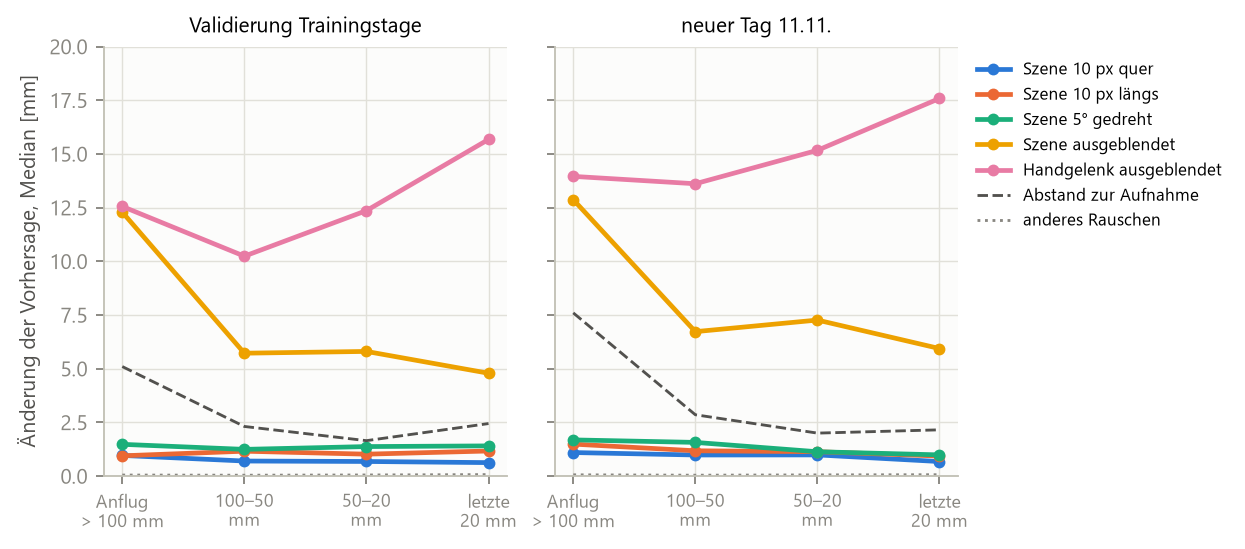
\includegraphics[width=\textwidth]{versuche/kamera_empfindlichkeit.png}
  \caption[Empfindlichkeit der Policy gegenüber Bildstörungen]{Änderung der Vorhersage
  (Median) je Phase der Fahrt und Art der Bildstörung.}
  \label{fig:kamera}
\end{figure}

% ==============================================================================
\section{Drehbias der Demonstrationen}
\label{sec:drehbias}

\paragraph{Frage.} An der Anlage drehte C2 bei Lagen, die eine Drehung nach minus verlangen,
im Median \ang{31} zu wenig (8 Fahrten), bei Plus-Lagen nur \ang{3}. Woran liegt das?

\paragraph{Vorgehen.} Auswertung der Drehungen in den Demonstrationen und zwei Varianten mit
denselben Daten: C3 zieht Minus-Episoden im Training \num{2.83}-mal häufiger, C3a lässt
238 Plus-Episoden weg. Vergleich offline an den Anlagensituationen und in der \ac{vm}
\quelle{Berichte/2026-11-17_Drehbias_C3.pdf}.

\paragraph{Ergebnis.}
\begin{itemize}
  \item Die Demonstrationen waren einseitig: \SI{62}{\percent} Plus-, \SI{25}{\percent}
    Minus-Drehungen, im Mittel \ang{+38.8} (\cref{fig:drehbias}). Ursache war die
    Verteilung der Drehung um die geteachte Lage statt um die Startstellung
    (\cref{sec:lagen}).
  \item Gewichten (C3) wirkt besser als Ausdünnen (C3a): C3 will bei Minus-Lagen im Median
    \ang{15} mehr drehen, C3a nur \ang{9} und verliert durch die fehlenden Daten an
    Genauigkeit.
  \item Der Bias ist nur ein Teil der Ursache. Die ganze Drehung geschieht in der Gelenkfahrt
    bis \code{ANFLUG}; darunter dreht keine Demonstration mehr, und die Policy holt fehlende
    Drehung nicht nach. Außerdem kommandiert sie etwa \SI{35}{\percent} größere Schritte als
    die Demonstrationen, und der Arm folgt schlechter.
  \item Keiner der Tests ohne Anlage koppelt die Bilder an die Bewegung zurück; keiner konnte
    den Drehfehler deshalb zuverlässig vorhersagen.
\end{itemize}

\begin{figure}[htbp]
  \centering
  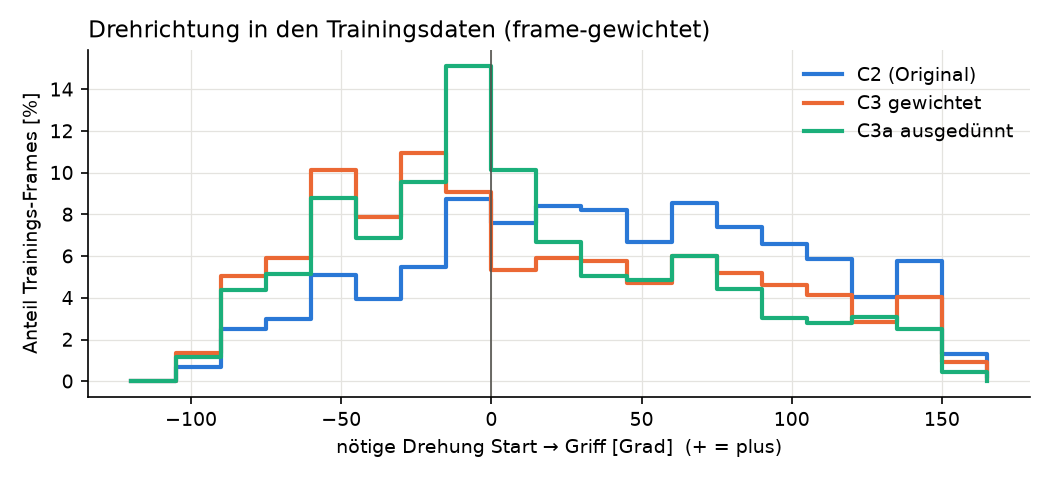
\includegraphics[width=0.85\textwidth]{versuche/drehbias_verteilung.png}
  \caption[Verteilung der Drehungen in den Demonstrationen]{Verteilung der nötigen Drehung
  zwischen Start und Griff in den 602 Demonstrationen.}
  \label{fig:drehbias}
\end{figure}

% ==============================================================================
\section{Folgerungen für den neuen Datensatz}
\label{sec:folgerungen}

Aus den Versuchen bis zum 17.11.\ wurden die Standards für den nächsten Datensatz abgeleitet
und im Code umgesetzt:
\begin{itemize}
  \item Drehung der Lagen um die Startstellung verteilt (Drehbias),
  \item Endanflug \SI{0.02}{\metre\per\second} (mehr Bilder kurz vor dem Bauteil),
  \item gezielter seitlicher und Drehversatz im Anflug (Zögern und Abdriften unter
    \code{PRE_PICK}, \cref{sec:versatz}),
  \item Kameralicht an der Handgelenkkamera und fester Weißabgleich,
  \item erste Lage aus der Objekterkennung von Modul~1,
  \item Aufnahme nur bis zum Griff (Ablauf \code{pick_bis_griff}, seit 19.11.): Nach dem Griff
    hebt der Arm an und fährt an einen gemeinsamen Endpunkt \SI{15}{\centi\metre} über der
    Tischmitte statt zur Prüfvorrichtung. Das folgt aus dem Ergebnis von C und C$'$, spart Zeit
    je Episode und beim Zurücklegen. Der Endpunkt muss für alle Lagen gleich sein, damit die
    Rückfahrt zur nächsten Lage passt. Bei der Ausführung plant dann der Planer den Transport
    zum Übergabepunkt.
\end{itemize}

% ==============================================================================
\section{Weitere Versuche}
\label{sec:weitere-versuche}

\todo[inline]{Platz für die Ergebnisse mit dem neuen Datensatz (ab 19.11.), den Gegenversuch
mit C3 an der Anlage und \acs{dagger}.}

\chapter{Diskussion}
\label{ch:diskussion}

\todo[inline]{Vorläufige Fassung auf dem Stand vom 19.11. Nach den Versuchen mit dem neuen
Datensatz überarbeiten.}

% ==============================================================================
\section{Bewertung der Designentscheidungen}
\label{sec:bewertung}

\Cref{tab:bewertung} stellt die wichtigsten Entscheidungen ihrer Wirkung in den Versuchen
gegenüber.

\begin{table}[htbp]
  \centering
  \caption{Designentscheidungen und ihre Bewertung nach den Versuchen}
  \label{tab:bewertung}
  \small
  \begin{tabularx}{\textwidth}{@{}>{\raggedright\arraybackslash}p{38mm} X@{}}
    \toprule
    Entscheidung & Bewertung \\
    \midrule
    Ports und Adapter, hardwarefrei entwickelt & bewährt: Die Kette lief vor dem ersten
      Anlagentag vollständig; an der Anlage blieben nur Adapter- und Physikthemen. \\
    Planer statt Teleoperation & bewährt: gleichmäßiges Tempo und über 700 Demonstrationen
      mit wenig Handarbeit. Nachteil: Alle Bahnen haben dieselbe Struktur; was der Planer nie
      zeigt (z.\,B.\ Drehen unter \code{ANFLUG}), kann die Policy nicht. \\
    Rauschen mit Trichter & in der Vorstudie deutlich wirksam. An der Anlage zeigte sich die
      Lücke im Endanflug, die der gezielte Versatz schließen soll. \\
    Absolute Gelenkwinkel als Aktion & bewährt: direkte Abbildung auf \code{servo_j}, keine
      Drift durch aufsummierte Änderungen. \\
    Direkte Vorhersage der Aktionsfolge & notwendig: Mit Rauschvorhersage waren zehn
      Entrauschungsschritte zu ungenau. \\
    \code{servo_j} mit Override \num{0.5} & bewährt: ruhig wie ein Herstellerprogramm und
      bahntreu. \\
    Keine Rektifizierung & bestätigt: Die Policy reagiert kaum auf die Kameralage. \\
    Eigene Sicherheitsschicht & notwendig: In der \acs{vm} wäre die Werkzeugspitze in gut der
      Hälfte der Fahrten unter den Tisch gegangen. Die Stufen sind jeweils aus einem
      beobachteten Fehlerfall entstanden. \\
    Policy nur für den Griff & vielversprechend: weniger Abbrüche und Tischfahrten, gleiche
      Genauigkeit. \\
    \bottomrule
  \end{tabularx}
\end{table}

% ==============================================================================
\section{Grenzen}
\label{sec:grenzen}

\paragraph{Aussagekraft der Tests ohne Anlage.} Weder der Offline-Test noch der \ac{vm}-Test
koppeln die Bilder an die Bewegung zurück. Sie eignen sich zum Vergleich von Modellen und zum
Finden grober Fehler, sagen aber die Genauigkeit an der Anlage nur ungefähr und den Drehfehler
gar nicht vorher. Der einzige vollständige Test ist die Anlage, an der aus Zeit- und
Sicherheitsgründen nur wenige Fahrten möglich waren.

\paragraph{Fehlerfortpflanzung bleibt.} Offline ist die Policy auf wenige Millimeter genau, an
der Anlage auf knapp einen Zentimeter. Der Unterschied entsteht in Zuständen, die sie selbst
herbeiführt. Das ist genau die Hürde aus \cref{sec:covariate-shift}; das eingespeiste
Rauschen verringert sie, beseitigt sie aber nicht dort, wo es gedämpft ist.

\paragraph{Ungeklärte Verschlechterung.} Warum die Daten vom 11.11.\ die Genauigkeit
verschlechterten, ist offen. Der Befund zeigt, wie empfindlich das Ergebnis auf schwer
greifbare Unterschiede der Aufnahmebedingungen reagiert.

\paragraph{Umfang.} Alle Versuche verwenden ein Bauteil auf einem ebenen Tisch, ohne Kiste und
ohne Störungen während der Fahrt. Aussagen über andere Bauteile oder Szenen sind daraus nicht
ableitbar.

\chapter{Fazit und Ausblick}
\label{ch:fazit}

% ==============================================================================
\section{Fazit}
\label{sec:fazit}

\todo[inline]{Ergebnis steht noch aus. Nach den Versuchen mit dem neuen Datensatz schreiben:
Erfolgsquote an der Anlage, Genauigkeit, Vergleich mit dem klassischen Greifen von Modul~2.}

Bis zum Stand dieses Dokuments ist die vollständige Kette aus automatischer Aufnahme mit
eingespeistem Rauschen, Training einer Diffusion Policy und sicherer Ausführung umgesetzt und
in das Gesamtsystem eingebunden. An der Anlage findet die Policy das Bauteil an unbekannten
Lagen aus den Bildern und trifft den Greifpunkt im Median auf knapp \SI{1}{\centi\metre}.
Die verbleibenden Fehler entstehen im Endanflug und bei der Drehung, in Zuständen, die die
Demonstrationen nicht abdecken.

% ==============================================================================
\section{Ausblick}
\label{sec:ausblick}

\paragraph{DAgger.} Die Fehler an der Anlage entstehen dort, wo die Demonstrationen keine
Beispiele haben. Genau diese Zustände sammelt \ac{dagger} (\cref{sec:covariate-shift}). Da der
Experte in Modul~4 ein Planer ist, kann er jeden Zustand nachträglich beschriften: Bei
bekannter Lage ist die richtige Aktion \enquote{von hier senkrecht über den Greifpunkt, dann
ab}. Geplant ist, Fahrten der Policy mit Bildern aufzuzeichnen, offline mit den Aktionen des
Planers zu beschriften und im Training höher zu gewichten. Erste Episoden dieser Art wurden am
17.11.\ aufgenommen \quelle{Dokumentation/DAgger-Ablauf.md}.

\paragraph{Weitere Punkte.}
\begin{itemize}
  \item Gegenversuch mit dem gewichteten Modell C3 an den Minus-Lagen,
  \item Drehkorrektur unterhalb von \code{ANFLUG} lehren und die Drehfahrt verlangsamen,
  \item geordneter Abbruch aus dem Ablauf des Gesamtsystems,
  \item Vergleich nur mit Handgelenkkamera, da der Datensatz beide Bildströme enthält,
  \item Übertragung auf weitere Bauteile und auf das Greifen aus einer Kiste.
\end{itemize}


\printbibliography[heading=bibintoc,title=Literaturverzeichnis]

\appendix
\chapter{Wichtige Parameter}
\label{app:parameter}

Alle Konstanten stehen mit Begründung in \code{bc/config.py}. \Cref{tab:parameter} fasst die
zusammen, die in diesem Dokument vorkommen.

\begin{table}[htbp]
  \centering
  \caption{Wichtige Parameter (Stand 19.11.2026)}
  \label{tab:parameter}
  \small
  \begin{tabularx}{\textwidth}{@{}l l X@{}}
    \toprule
    Name in \code{config.py} & Wert & Bedeutung \\
    \midrule
    \code{CONTROL_RATE_HZ} & \SI{15}{\hertz} & Takt von Aufnahme und Policy \\
    \code{SERVO_RATE_HZ} & \SI{60}{\hertz} & Sollwertstrom \code{servo_j} \\
    \code{TRANSIT_SPEED_MS} & \SI{0.15}{\metre\per\second} & Transfer, linear \\
    \code{APPROACH_SPEED_MS} & \SI{0.02}{\metre\per\second} & Endanflug \\
    \code{PTP_JOINT_SPEED_RADS} & \SI{0.5}{rad/s} & Gelenkfahrt \\
    \code{SEGMENT_RAMP_S} & \SI{0.5}{\second} & Anfahr- und Bremsrampe \\
    \code{GRIPPER_DWELL_S} & \SI{0.5}{\second} & Wartezeit nach Greiferbefehl \\
    \code{NOISE_TRANS_AMPLITUDE_M} & \SI{15}{\milli\metre} & Rauschen Position \\
    \code{NOISE_ROT_AMPLITUDE_RAD} & \SI{0.05}{rad} & Rauschen Drehung \\
    \code{NOISE_OU_TAU_S} & \SI{0.8}{\second} & Zeitkonstante \\
    \code{FUNNEL_START_DIST_M} / \code{_ZERO_} & \SI{15}{} / \SI{2}{\centi\metre} & Trichter \\
    \code{APPROACH_OFFSET_SHARE} & \num{0.5} & Anteil Episoden mit Versatz \\
    \code{COLLISION_MARGIN_M} & \SI{3}{\centi\metre} & Sicherheitsabstand \\
    \code{SYNC_MAX_SKEW_S} & \SI{30}{\milli\second} & Zeitbudget Bild--Zustand \\
    \code{AUTO_YAW_RANGE_DEG} & \ang{\pm 45} & Drehung neuer Lagen \\
    \code{POLICY_HORIZON} / \code{_N_ACTION_STEPS} & 16 / 8 & Vorhersagehorizont \\
    \code{POLICY_INFERENCE_STEPS} & 10 & \acs{ddim}-Schritte \\
    \code{POLICY_MAX_JOINT_SPEED_RADS} & \SI{0.8}{rad/s} & weiche Begrenzung \\
    \code{SERVO_MAX_JOINT_SPEED_RADS} & \SI{1.0}{rad/s} & harte Grenze \\
    \code{INFER_MAX_FRAME_AGE_S} & \SI{100}{\milli\second} & Höchstalter eines Bildes \\
    \code{PROBE_GAP_M} & \SI{25}{\milli\metre} & Abstand beim Probegriff \\
    \bottomrule
  \end{tabularx}
\end{table}

\chapter{Verzeichnis der Berichte und Einzeldokumente}
\label{app:berichte}

Die folgenden Unterlagen liegen unter \code{code/m4_behavior_cloning/} und bleiben als
eigenständige Dokumente bestehen.

\begin{table}[htbp]
  \centering
  \caption{Berichte (\code{Berichte/})}
  \label{tab:berichte}
  \small
  \begin{tabularx}{\textwidth}{@{}l X l@{}}
    \toprule
    Datum & Inhalt & Abschnitt \\
    \midrule
    16.09. & Rauschstudie ohne Bilder; Rauschen je Episode in der \acs{vm} & \ref{sec:rauschstudie} \\
    17.09. & Durchstich der Kette in Simulation und \acs{vm} & \ref{sec:durchstich} \\
    01.--21.10. & Labortage: Systemcheck, Aufruflatenz, Sollwerttakt, Trajektorienpuffer,
      Servo-Strom, Kinematik, Smartphone-Messungen & \ref{sec:labortage} \\
    10.11. & Modellprüfung Checkpoint 09.11. & \ref{sec:modellpruefung} \\
    13.11. & \acs{vm}-Test mit den Aufnahmen vom 11.11. & \ref{sec:replay-1111} \\
    13.--15.11. & Versuchsreihe Policy-Varianten & \ref{sec:varianten} \\
    16.11. & Anlagentest C2 & \ref{sec:anlagentest-c2} \\
    16.11. & Kameraempfindlichkeit C2 & \ref{sec:kamera-empfindlichkeit} \\
    17.11. & Drehbias C2/C3/C3a & \ref{sec:drehbias} \\
    \bottomrule
  \end{tabularx}
\end{table}

\begin{table}[htbp]
  \centering
  \caption{Einzeldokumente (\code{Dokumentation/} und \code{Requierments/})}
  \label{tab:einzeldokumente}
  \small
  \begin{tabularx}{\textwidth}{@{}l X@{}}
    \toprule
    Dokument & Inhalt \\
    \midrule
    \code{requierments.md} & Anforderungen und Entscheidungen je Arbeitspaket \\
    \code{Kamera-Inbetriebnahme.md} & Kameras: Hardware, SDK, Einstellungen, Mechanik \\
    \code{Taktzeit-und-RPC-Latenz.md} & Eingrenzung abbrechender Bahnen, Messmethode \\
    \code{Zittern-an-der-Anlage.md} & Ursache und Lösung des Zitterns, alle Messreihen \\
    \code{Training-und-Inferenz.md} & Export, Training, Ausführung, Prüfung ohne Anlage \\
    \code{DAgger-Ablauf.md} & geplanter Ablauf für \acs{dagger} \\
    \code{Environment-*.md} & Einrichtung der Python-Umgebungen \\
    \code{Anlagentag-Checkliste.md} & Ablauf eines Tages an der Anlage \\
    \bottomrule
  \end{tabularx}
\end{table}


\end{document}
